%% Comment 4:	Mechanisms

%I encourage the authors to expand the discussion of mechanisms, that at present is not very well developed. First, the authors should be explicit on what they mean with “police effectiveness”. Typically, effectiveness is proxied by arrests or clearance rates. This would also help separate two channels: deterrence and police effectiveness. Deterrence would change the incentives to commit crime, and thus would be reflected in reductions in crime, whereas the latter would be reflected in the ability of the police to deal with crime, which would show up in arrests conditional on crime. Furthermore, to shed light on this, it would be useful to consider whether the reform affected response times, patrolling patterns, or any other proxies that capture the ability of the police to solve crime, such as improved technology. An alternative channel is that the reform increased the salience of policing and thus raised citizen awareness. For instance, was the policy advertised? Of course, these mechanisms are not mutually exclusive, and I recognize that disentangling them empirically may be difficult, but a more systematic discussion would be very valuable.

Thanks for the specific and clear guidance to improve the analysis of mechanisms.

We revised the manuscript so that the mechanism discussion now distinguishes more clearly between deterrence and police effectiveness as two conceptually distinct but empirically intertwined channels through which beat policing may improve public safety and security perceptions. In the revised framing, police effectiveness is no longer used as a label for the main outcomes; instead, it refers to the capacity of police to prevent and resolve crime. In practice, with our data we cannot cleanly separate how much of the total effect comes from each channel, because they can reinforce each other: stronger preventive action and higher police presence can deter crime, and improved capacity to solve crimes can also deter crime by increasing the expected probability of apprehension; at the same time, lower crime incidence may allow police to concentrate effort on crime resolution. While we were not granted access to patrolling patterns or response times, we provide evidence consistent with both channels operating. Specifically, \emph{Plan Cuadrante} increases perceived police presence (Panel (a) of Figure \ref{fig:police_performance}), reduces household victimization and reported crime (Panels (a) and (b) of Figure \ref{fig:figure02}), increases arrests (Panel (c) of Figure \ref{fig:police_performance}), and increases arrests per reported crime (Panel (d) of Figure \ref{fig:police_performance}). The latter result should nonetheless be interpreted with caution, as the composition of reported crimes may also change with the program, affecting the ratio independently of any change in police effectiveness. Accordingly, in Section 4.4 the focus is not to isolate deterrence from effectiveness, but to disentangle which components of \emph{Plan Cuadrante}---resources, territorial deployment, and policing strategy---are most likely to explain the effects we document.

Regarding the possibility that the reform was accompanied by an advertisement campaign that increased the salience of policing and raised citizen awareness, we believe this is unlikely for two reasons. First, \emph{Plan Cuadrante} was an internal operational reform of Carabineros with no formal public communication component in its design. While the program received some media attention when it was broadly rolled out across Santiago in 2000, we find no evidence of targeted information campaigns at the municipality level when individual municipalities subsequently joined the program, and the staggered rollout over more than a decade makes a sustained media salience mechanism implausible. Second, and more importantly, if the improvement in crime were driven by media coverage or information campaigns, one would expect the effects to be concentrated shortly after adoption and to fade over time. Instead, the dynamic estimates show that the effects for most outcomes grow and persist over time.


Below we provide the updated mechanism section:

\begin{adjustwidth}{2em}{0em}
{\setcounter{figure}{3}\renewcommand{\thefigure}{\arabic{figure}}
%\textbf{4.4 What Is Driving the Effects of \emph{Plan Cuadrante}?}


To reduce crime and improve security perceptions, police forces need to strengthen both prevention and police effectiveness. Both margins can be shaped by resources, territorial deployment, and policing strategy. This section examines which components of \emph{Plan Cuadrante} are most likely to drive the effects documented in Section \ref{results}. 

The central objective of \emph{Plan Cuadrante} was to introduce a beat policing model by reorganizing deployment. Police operational territories that had typically matched municipal boundaries were subdivided into quadrants, and officers were permanently assigned to these quadrants. During our study period, national operational guidelines remained the same in adopting and non-adopting municipalities. Still, this new deployment likely affected policing strategy at a more operational level, because it allowed officers to adapt patrol routes, schedules, and prevention practices using the local knowledge that the program sought to build.

Although changes in resources were not the core of the reform, implementation contemplated increases in municipalities that lacked the personnel and patrol capacity required to move to this model. During the period we study, Chile was expanding public spending on security, and police resources increased in most municipalities regardless of whether or when they adopted \emph{Plan Cuadrante}. On average, however, municipalities adopting the program experienced larger increases in officers and patrol vehicles, as shown in panels (a) and (b) of Figure \ref{fig:resources}. Since increases in police resources have been shown to reduce crime in some contexts \citep{Evans}, this pattern raises a central question for interpretation, namely whether our estimates reflect resource expansion or the deployment and strategy changes introduced by \emph{Plan Cuadrante}. We address this question through a set of exercises that exploit heterogeneity in resource increases across municipalities and over time.

\FloatBarrier
%--- Implementation
\begin{figure}[H]
    \centering
    \caption{Plan Cuadrante and Changes in Police Resources}
    \label{fig:resources}
    \label{fig:figure_resources}
    \begin{tabular}{cc}
        \begin{minipage}[t]{0.48\textwidth}
            \centering
            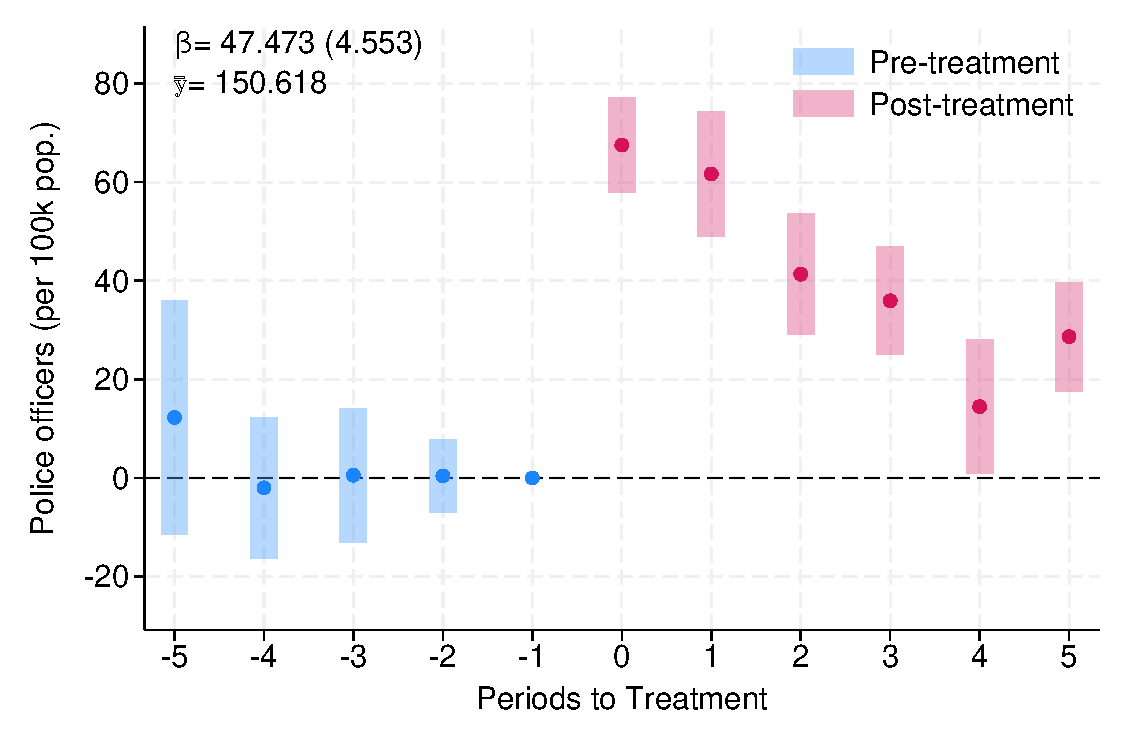
\includegraphics[width=\linewidth]{../manuscript/Graphs/fig4_officers.pdf}

            \small (a) Effect on the number of police officers
        \end{minipage}
        &
        \begin{minipage}[t]{0.48\textwidth}
            \centering
            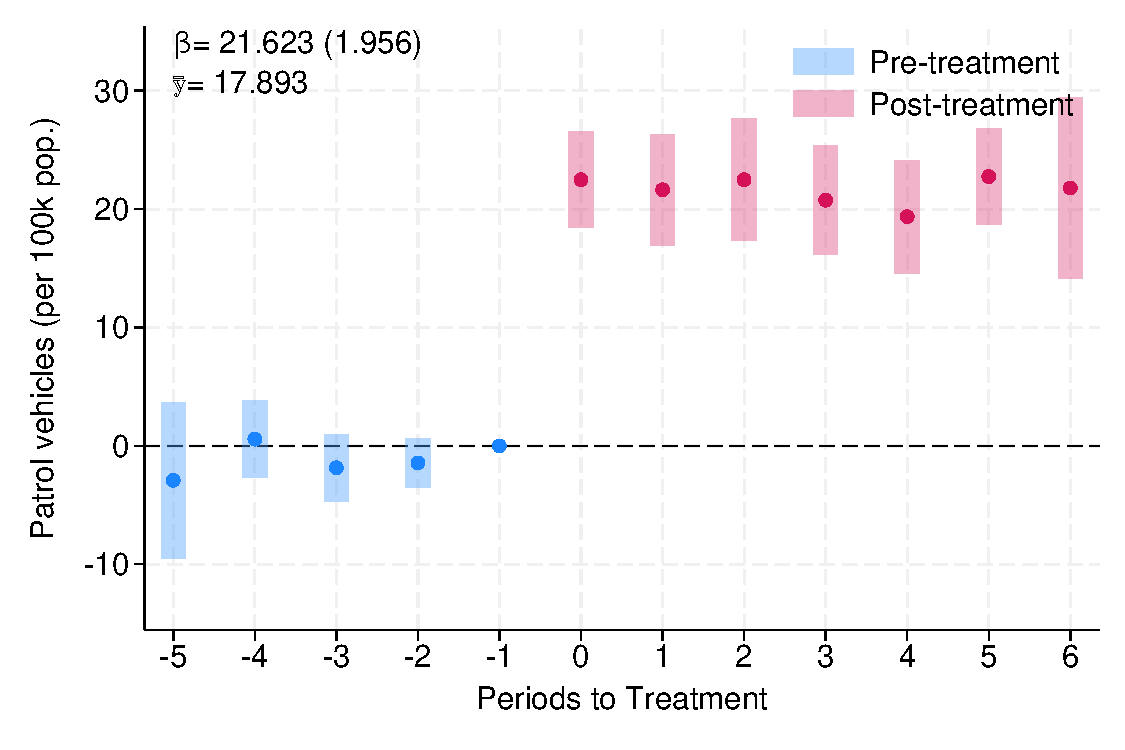
\includegraphics[width=\linewidth]{../manuscript/Graphs/fig4_patrols.pdf}

            \small (b) Effect on the number of patrol vehicles
        \end{minipage}
        \\[4pt]
        \begin{minipage}[t]{0.48\textwidth}
            \centering
            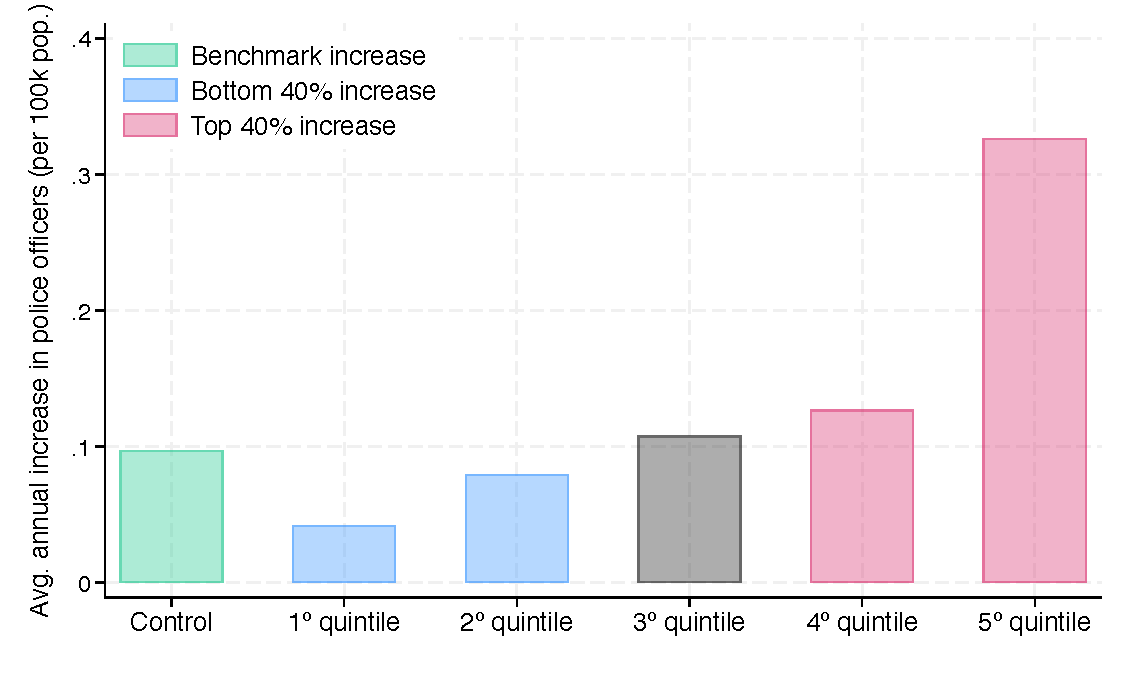
\includegraphics[width=\linewidth]{../manuscript/Graphs/increase_enusc_off_quintiles.pdf}

            \small (c) Distribution of $\Delta$ in police officers
        \end{minipage}
        &
        \begin{minipage}[t]{0.48\textwidth}
            \centering
            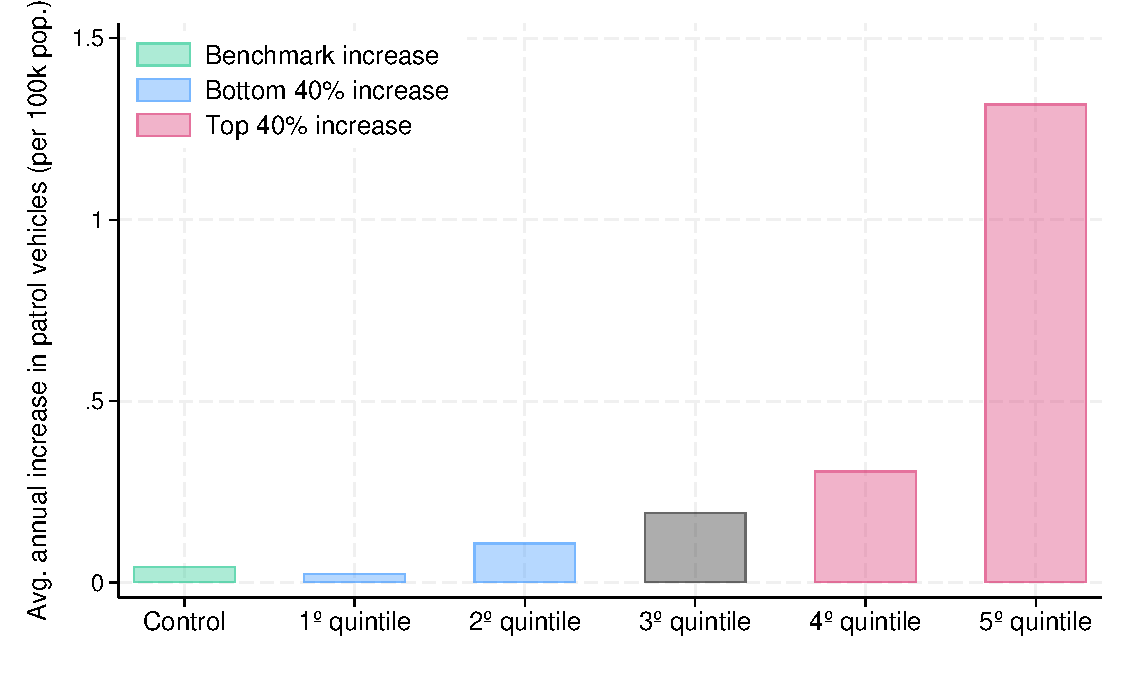
\includegraphics[width=\linewidth]{../manuscript/Graphs/increase_enusc_pv_quintiles.pdf}

            \small (d) Distribution of $\Delta$ in patrol vehicles
        \end{minipage}
        \\[4pt]
        \begin{minipage}[t]{0.48\textwidth}
            \centering
            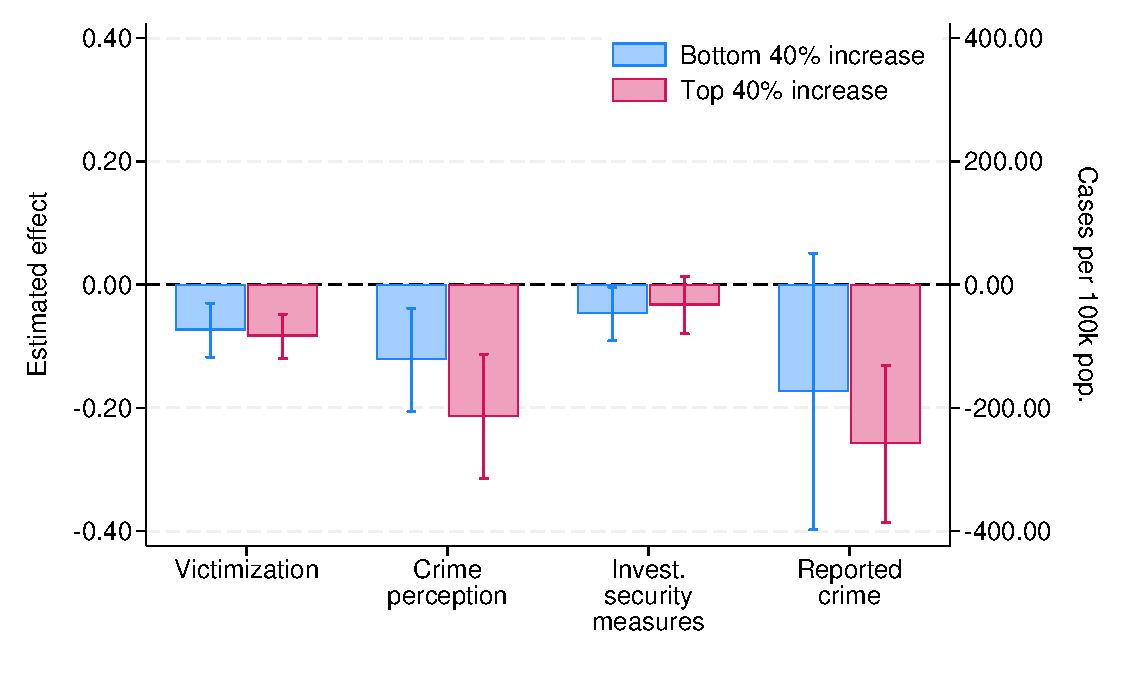
\includegraphics[width=\linewidth]{../manuscript/Graphs/heterogeneity_off.pdf}

            \small (e) Effects by the intensity of $\Delta$ in police officers
        \end{minipage}
        &
        \begin{minipage}[t]{0.48\textwidth}
            \centering
            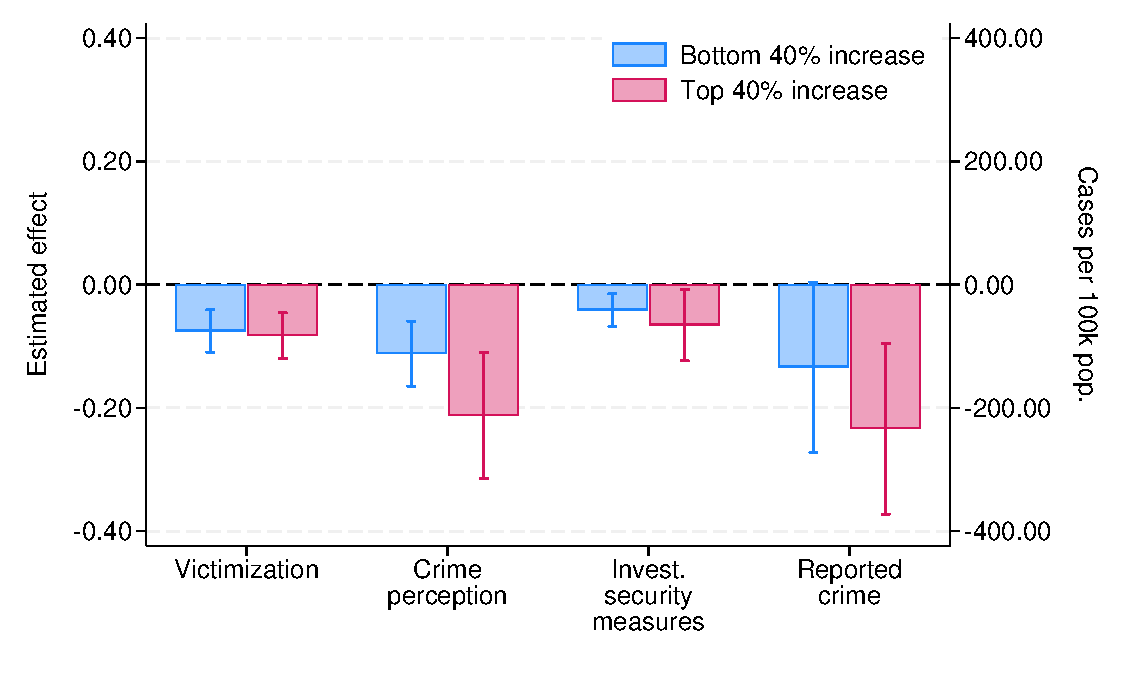
\includegraphics[width=\linewidth]{../manuscript/Graphs/heterogeneity_pv.pdf}

            \small (f) Effects by the intensity of $\Delta$ in patrol vehicles
        \end{minipage}
    \end{tabular}
    \vspace{4pt}
    \begin{minipage}{0.99\textwidth}
    \footnotesize Notes: Panels (a) and (b) show the effect of \emph{Plan Cuadrante} on police officers and patrol vehicles per 100,000 inhabitants. Panels (c) and (d) show the distribution of annual changes in officers and patrol vehicles across municipalities. Panels (e) and (f) report effects by the intensity of resource changes, comparing municipalities in the bottom 40\% and top 40\% of the distribution. The estimation follows \citet{Callaway}. The graphs display estimated coefficients and 95\% confidence intervals. Standard errors are clustered at the municipality level using wild bootstrapping.
    \end{minipage}
\end{figure}
\FloatBarrier
Panels (c) and (d) of Figure \ref{fig:resources} show that the average increase in police resources masks substantial heterogeneity. Municipalities in the bottom 40\% of the resource-change distribution (blue bars) experienced increases close to the average annual variation observed among never treated and not-yet-treated municipalities (green bar). By contrast, municipalities in the top 40\% (red bars) experienced much larger increases, with officers rising by around 22\% and patrol vehicles by around 80\%. If the effects of \emph{Plan Cuadrante} were driven by resource increases alone, we would not expect effects in municipalities whose resource increases were similar to those of the control group. Yet panels (e) and (f) of Figure \ref{fig:resources} show sizeable effects for most crime and crime-perception outcomes even in that low-increase group. While there may be a resource gradient for some crime-perception outcomes, the effects on twelve-month victimization and private investment in security among municipalities with control-like resource increases are close in magnitude to those in municipalities with larger increases. Reassuringly, municipalities in the top and bottom 40\% of the resource-increase distribution do not display differential pre-treatment trends in outcomes or police resources, which suggests that this heterogeneity is not driven by differential pre-existing trends.\footnote{We test for the joint significance of the pre-treatment coefficients between the two groups, separately for the split based on the increase in police officers and the split based on the increase in patrol vehicles. The resulting p-values are, respectively, 0.823 and 0.048 for victimization, 0.059 and 0.379 for crime perception, 0.820 and 0.157 for investment in security measures, and 0.213 and 0.419 for reported crime, as well as 0.616 and 0.444 for police officers and 0.405 and 0.157 for patrol vehicles.}

Although we cannot fully separate the beat policing component from the resource component of the reform---resources may have been important to enable effective implementation of the program, or may explain part of the effects in some municipalities---the fact that municipalities with resource increases similar to those experienced by control municipalities still display sizeable effects indicates that the effects of \emph{Plan Cuadrante} are not driven entirely by resources.\footnote{We also re-estimate the results in Figure \ref{fig:figure02} but controlling for police resources. Online Appendix Table \ref{tab:results_controlbyresources} shows that the magnitude of the estimated effects remains similar for most variables, although the statistical significance is reduced in some estimations. This likely reflects a mechanical feature of the \citet{Callaway} estimation procedure: control variables are not incorporated parametrically, but are instead used to construct the comparison group via outcome regression or propensity-score weighting, so the resulting estimation uncertainty propagates to the ATT standard errors. Note, in addition, that police resources are a bad control---i.e., at least part of their variation is a result of the adoption of \emph{Plan Cuadrante}---so these results should be interpreted cautiously.}\footnote{Table \ref{tab:resourcecorrelates} in Online Appendix \ref{sec:appendixB} examines which factors are associated with a larger increase in police resources upon the adoption of \emph{Plan Cuadrante}.}


\FloatBarrier
%--- Implementation
\begin{figure}[h!]
    \centering
    \caption{Police Resources and Public Safety}
    \label{fig:resources2}
    \begin{subfigure}[t]{0.55\textwidth}
        \centering
        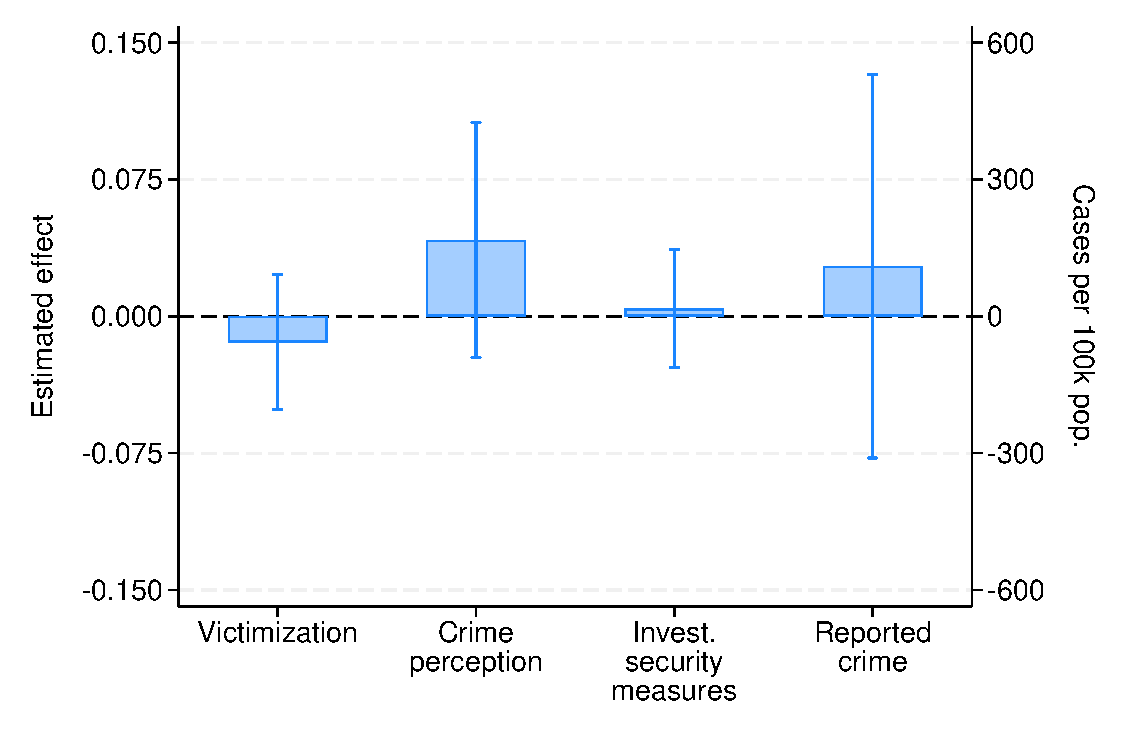
\includegraphics[width=\linewidth]{../manuscript/Graphs/results_SC_att_combined.pdf}
        \caption{Effects of \emph{Seguridad Ciudadana}}
    \end{subfigure}
    \\[6pt]
    \begin{subfigure}[t]{0.55\textwidth}
        \centering
        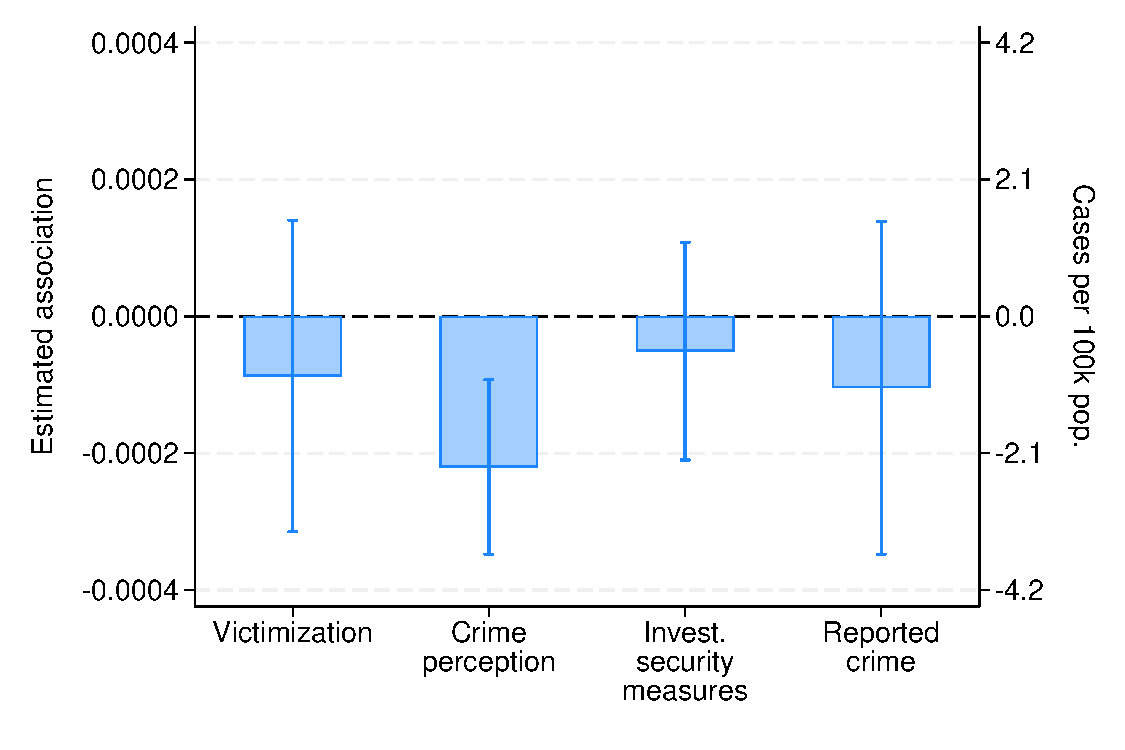
\includegraphics[width=\linewidth]{../manuscript/Graphs/results_corr_novariation_off_santiago.pdf}
        \caption{Association between police officers and effectiveness}
    \end{subfigure}
    \\[6pt]
    \begin{subfigure}[t]{0.55\textwidth}
        \centering
        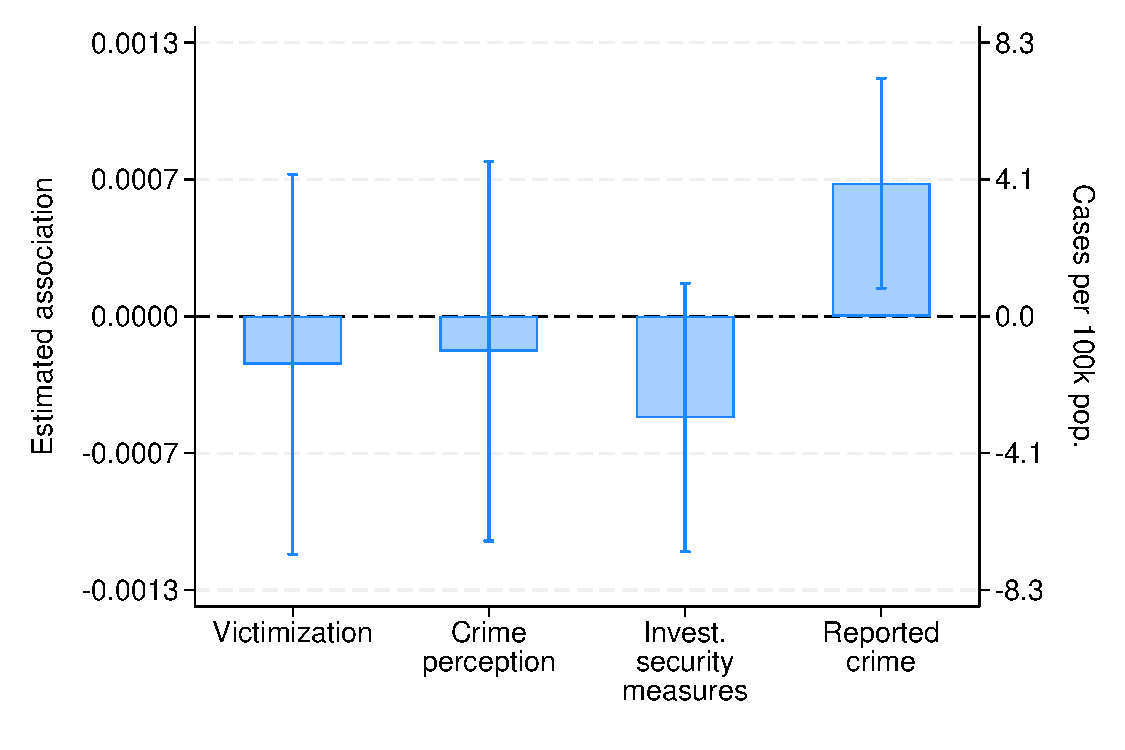
\includegraphics[width=\linewidth]{../manuscript/Graphs/results_corr_novariation_veh_santiago.pdf}
        \caption{Association between patrol vehicles and effectiveness}
    \end{subfigure}
    \\[8pt]
    \begin{minipage}{0.99\textwidth}
    \footnotesize Notes: Panel (a) reports the pooled effect of \emph{Seguridad Ciudadana}, a program that expanded local security personnel to support patrolling and deterrence but did not replicate the deployment-and-strategy features of \emph{Plan Cuadrante}. Panels (b) and (c) report within-municipality associations between police resources and police-effectiveness outcomes among the 41 municipalities of the Santiago Metropolitan Region, all of which had adopted \emph{Plan Cuadrante} by 2000. The regressions include municipality and year fixed effects. Standard errors are clustered at the municipality level using the wild bootstrapping procedure.
    \end{minipage}
\end{figure}
\FloatBarrier

To further investigate whether resource increases alone can explain our results, we assess the effects of \emph{Seguridad Ciudadana}, a program that expanded local security personnel to support patrolling and deterrence, but did not replicate the core deployment-and-strategy features of \emph{Plan Cuadrante}. Using a difference-in-differences specification following \citet{Callaway}, panel (a) of Figure \ref{fig:resources2} shows no significant effects of these resource changes on police effectiveness. Further details about this exercise and the corresponding event-study estimates are reported in Online Appendix \ref{sec:appendixB} and Online Appendix Figure \ref{fig:figureA5}. 


Finally, we study whether variation in police resources in municipalities that had already adopted \emph{Plan Cuadrante} improves public safety and security perceptions. Using ENUSC data and information on resources for 2006--2012 in the 41 municipalities of the Santiago Metropolitan Region---all of which had adopted \emph{Plan Cuadrante} by 2000---we exploit variation in officers and patrol vehicles that is unrelated to program adoption. Panels (b) and (c) of Figure \ref{fig:resources2} show the association between police resources and our main outcomes, conditional on municipality and year fixed effects. With one exception---the association between police officers and crime perception---none of these associations is statistically significant at conventional confidence levels. \footnote{Online Appendix Figure \ref{fig:figureA7B} reports the same exercise and also shows similar results for the broader set of municipalities that adopted \emph{Plan Cuadrante} before 2006 and never-treated municipalities (red bars); see Online Appendix \ref{sec:appendixB} for further details.}

Taken together, these results suggest that resource increases alone do not account for the effects of \emph{Plan Cuadrante}. We next turn to evidence that speaks more directly to the beat-policing components of the reform.

Panel (a) of Figure \ref{fig:police_performance} shows that, following the adoption of \emph{Plan Cuadrante}, households are much more likely to report increased police presence in their neighborhoods. The share of households perceiving increased police presence rises by 35 percentage points (156\%), the share reporting that police pass by their house daily rises by 22 percentage points (59\%), the share reporting never seeing police patrols near their house falls by 10 percentage points (57\%), and complaints about lack of police surveillance fall by around 5 percentage points (20\%). This evidence is consistent with both larger resources and the new deployment model. Yet the latter estimate---the only police-presence outcome for which we can separately estimate effects in municipalities with small and large resource increases---is similar in magnitude across the two groups, which suggests that the increase in police presence is not explained only by larger resource increases (see Online Appendix Figure \ref{fig:heterogeneity_appendix}).\footnote{We cannot estimate heterogeneous effects for other police-presence outcomes, such as the reporting of police passing by or the share of households perceiving an increase in police presence, because those variables are available only in ENUSC rounds 2003, 2005, and 2006, while resource data start in 2006.} More importantly, the broader pattern of results suggests that \emph{Plan Cuadrante} did more than simply increase patrolling intensity. Existing work shows that police presence can reduce crime while officers are present, but that its overall effects may be attenuated when crime is displaced across places or time windows \citep{MASTROBUONI2019, Blanes_Mastrobuoni_2018}. Our results point to something broader. As discussed in Section \ref{results}, we find actual declines in victimization and reported crime, together with no evidence of spillovers to neighboring municipalities. This pattern is more consistent with officers accumulating local knowledge and adapting prevention strategies to local conditions under stable territorial assignment than with a purely mechanical increase in patrol intensity.

Panel (b) of Figure \ref{fig:police_performance} reinforces this interpretation. Households in early-adopting municipalities report better police performance across multiple dimensions. They are 8.1 percentage points (16\%) more likely to rate police performance as good or very good, 7.6 percentage points (11\%) more likely to describe police as efficient, 5 percentage points (6\%) more likely to report that police are helpful, and 4.9 percentage points (7\%) more likely to report that police are well informed. They are also 3.9 percentage points (10\%) less likely to perceive police as corrupt, 7.9 percentage points (21\%) less likely to believe police fail to control crime, and 7.6 percentage points (22\%) less likely to report that police do not perform their duties effectively.\footnote{Information on police performance is only available in ENUSC round 2005. Using this round, we compare perceived police performance in municipalities that adopted \emph{Plan Cuadrante} in 2005 or earlier and in municipalities adopting after 2005. Figure \ref{fig:balance_doseresponse} in Online Appendix \ref{sec:appendixB} shows that the number of years of exposure to \emph{Plan Cuadrante} is positively correlated with perceived police performance. While these exercises on perceived police performance should be interpreted with caution, we show in the same appendix that the timing of future adoption is not correlated with perceived police performance in 2005 for municipalities that had not yet adopted the program by 2005.} %These perceived improvements are consistent with a setting in which officers become better informed about local routines and more effective in how they patrol and respond.

The administrative evidence points in the same direction. Panel (c) of Figure \ref{fig:police_performance} shows that arrests per 100,000 inhabitants increase by 48 (14\%) in our main estimates, even as crime declines overall.\footnote{As with reported crime, this event study is restricted to 5 pre-treatment and 7 post-treatment periods for symmetry with the ENUSC-based analysis; Online Appendix Figure \ref{fig:admin_uncapped} reports the results for arrests using the full set of pre-treatment and post-treatment periods.} This effect is also significant among municipalities with resource increases similar to those in the control group (see Online Appendix Figure \ref{fig:heterogeneity_appendix}). Consistent with this pattern, panel (d) of Figure \ref{fig:police_performance} shows that the arrest rate per reported crime also increases by 1.7 percentage points (10\%), suggesting that a higher share of crimes reported to the police are being solved. Because these gains appear even where resources did not increase more than in control municipalities, they are difficult to reconcile with a pure resource story and are more naturally interpreted as improvements in police effectiveness under the deployment and strategy changes introduced by \emph{Plan Cuadrante}. The corresponding event-study estimates for arrests, the arrest rate per reported crime, and trust in the police in Figure \ref{fig:police_performance} confirm that these changes emerge only after adoption.

Finally, panel (e) of Figure \ref{fig:police_performance} shows a sharp increase in trust in the police in our main specification (Section \ref{results}), consistent with one of the objectives of beat policing, namely bringing officers closer to the community and allowing them to accumulate local knowledge through repeated interaction. Online Appendix Figure \ref{fig:heterogeneity_appendix} shows that this effect remains sizeable both in municipalities that experienced resource increases similar to the control group and in those with larger increases.

Overall, although resources were likely important for implementation and may explain part of the effects in some municipalities, the results in this section indicate that resource changes alone are not enough to explain our findings. The evidence is more consistent with a combination of deployment changes and the strategy adjustments enabled by local knowledge accumulation under permanent assignment to quadrants.

\FloatBarrier
%--- Implementation
\begin{figure}[!ht]
    \centering
    \caption[\emph{Plan Cuadrante} and Changes in Police Performance]{\emph{Plan Cuadrante} and Changes in Police Performance}
    \label{fig:figure05}
    \label{fig:police_performance}
    \label{fig:effectiveness_es}
    \begin{subfigure}[t]{0.44\textwidth}
        \centering
        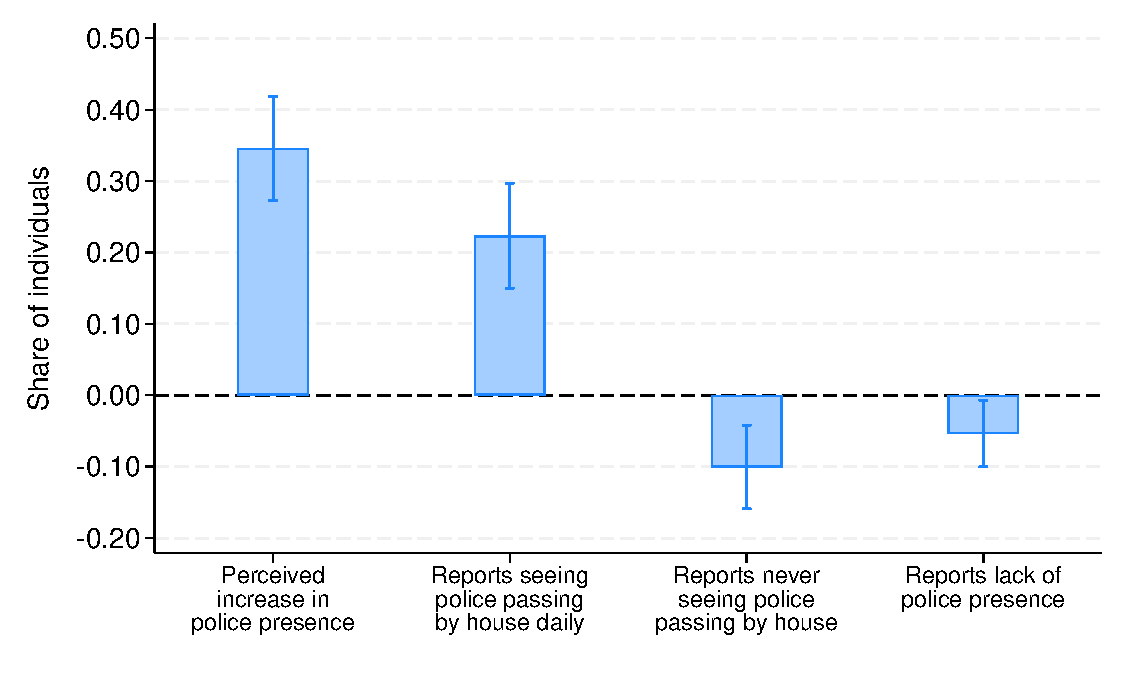
\includegraphics[width=\linewidth]{../manuscript/Graphs/results_policepresence.pdf}
        \caption{Effect on police presence}
    \end{subfigure}\hfill
    \begin{subfigure}[t]{0.44\textwidth}
        \centering
        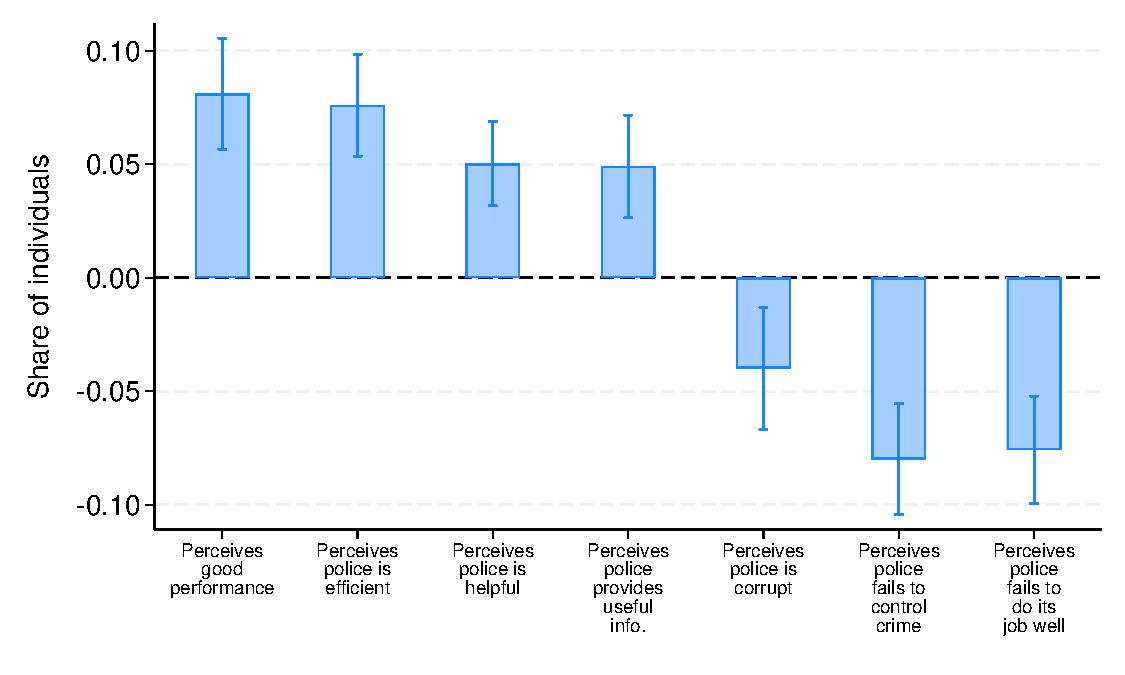
\includegraphics[width=\linewidth]{../manuscript/Graphs/combined_PCttest_2.pdf}
        \caption{Effect on perceived police performance}
    \end{subfigure}
    \\[6pt]
    \begin{subfigure}[t]{0.44\textwidth}
        \centering
        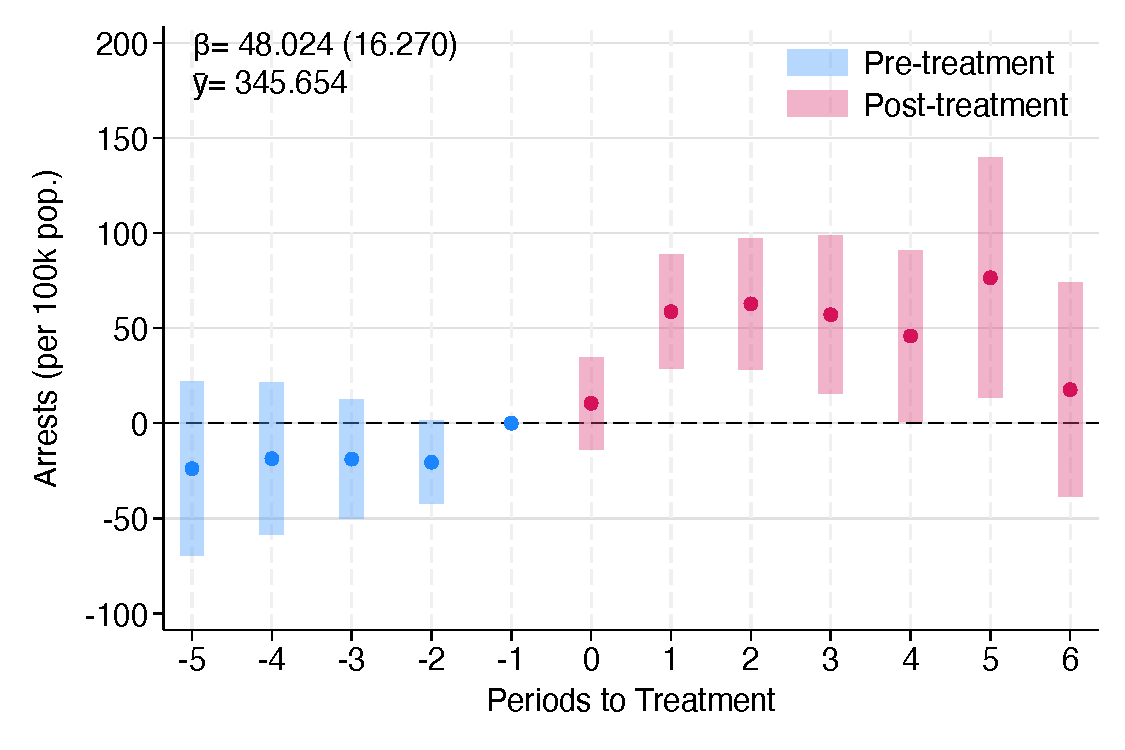
\includegraphics[width=\linewidth]{../manuscript/Graphs/totalarrestscrime_allcomunas.pdf}
        \caption{Arrests (per 100k pop.)}
    \end{subfigure}\hfill
    \begin{subfigure}[t]{0.44\textwidth}
        \centering
        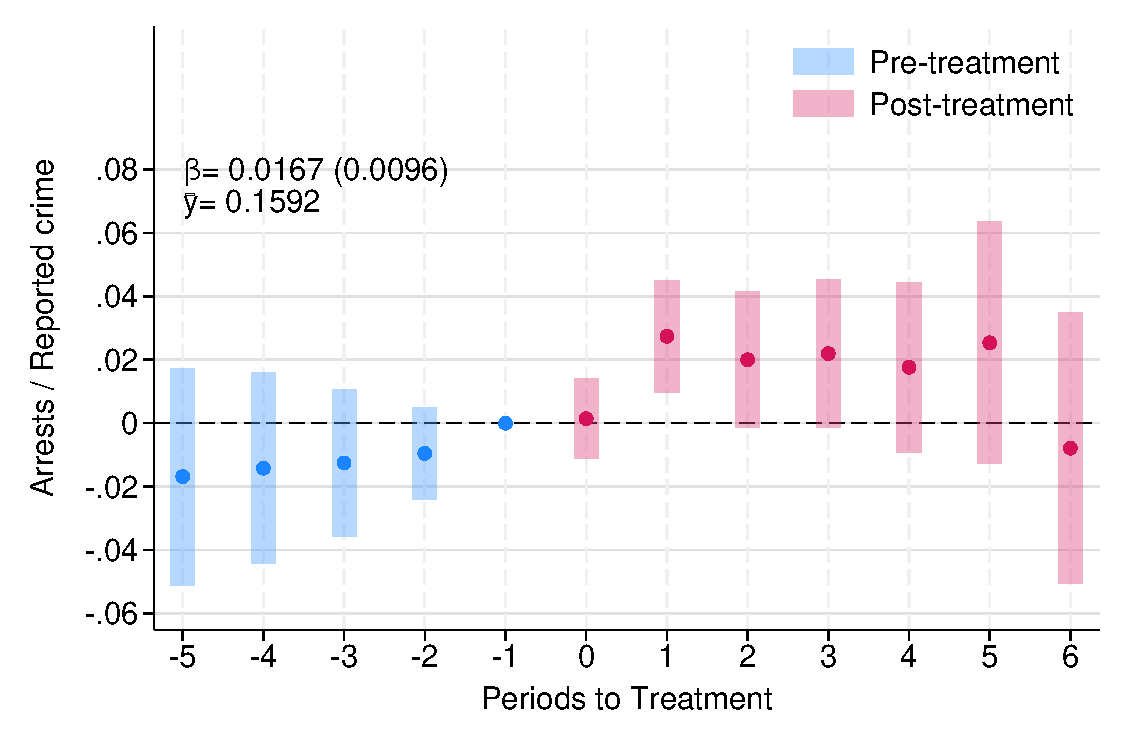
\includegraphics[width=\linewidth]{../manuscript/Graphs/arrests_over_reportedcrime_allcomunas.pdf}
        \caption{Arrests / Reported crime}
    \end{subfigure}
    \\[6pt]
    \begin{subfigure}[t]{0.44\textwidth}
        \centering
        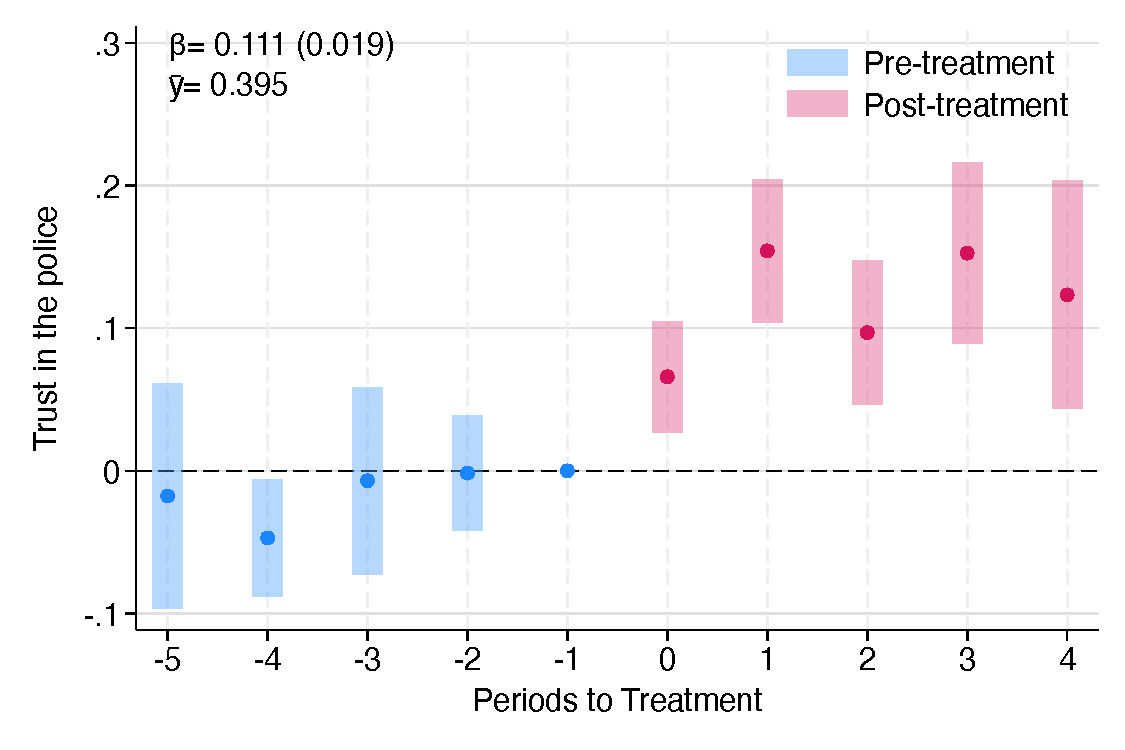
\includegraphics[width=\linewidth]{../manuscript/Graphs/results_trustcarabineros.pdf}
        \caption{Trust in the police}
    \end{subfigure}
    \\[8pt]
    \begin{minipage}{0.99\textwidth}
    \footnotesize Notes: Panel (a) reports the effects on perceived police presence. Panel (b) reports perceived police performance in 2005, comparing municipalities where \emph{Plan Cuadrante} was already implemented before 2006 with municipalities where it was implemented after 2005. Panels (c), (d), and (e) report dynamic event-study estimates for arrests per 100,000 inhabitants, the ratio of arrests to reported crime, and trust in the police. The estimation follows \citet{Callaway}. The graphs display estimated coefficients and 95\% confidence intervals. Standard errors are clustered at the municipality level using the wild bootstrapping procedure.
    \end{minipage}
\end{figure}

\FloatBarrier

%Overall, while resources were arguably important for implementation, the evidence suggests that the beat policing elements---permanent assignment of officers to quadrants and greater local knowledge---were important drivers of the improvements in public safety and security perceptions we document in the paper.



 
}
\end{adjustwidth}

\clearpage
\noindent\textbf{Other figures and tables referenced above:}
\vspace{0.5em}

{\setcounter{figure}{1}\renewcommand{\thefigure}{\arabic{figure}}
%--- Implementation
\begin{figure}[h!]
    \centering
    \caption{Effects of \emph{Plan Cuadrante} on Crime Outcomes and Security Perceptions}
    \label{fig:figure02}
    \begin{subfigure}{0.495\textwidth}
        \centering
        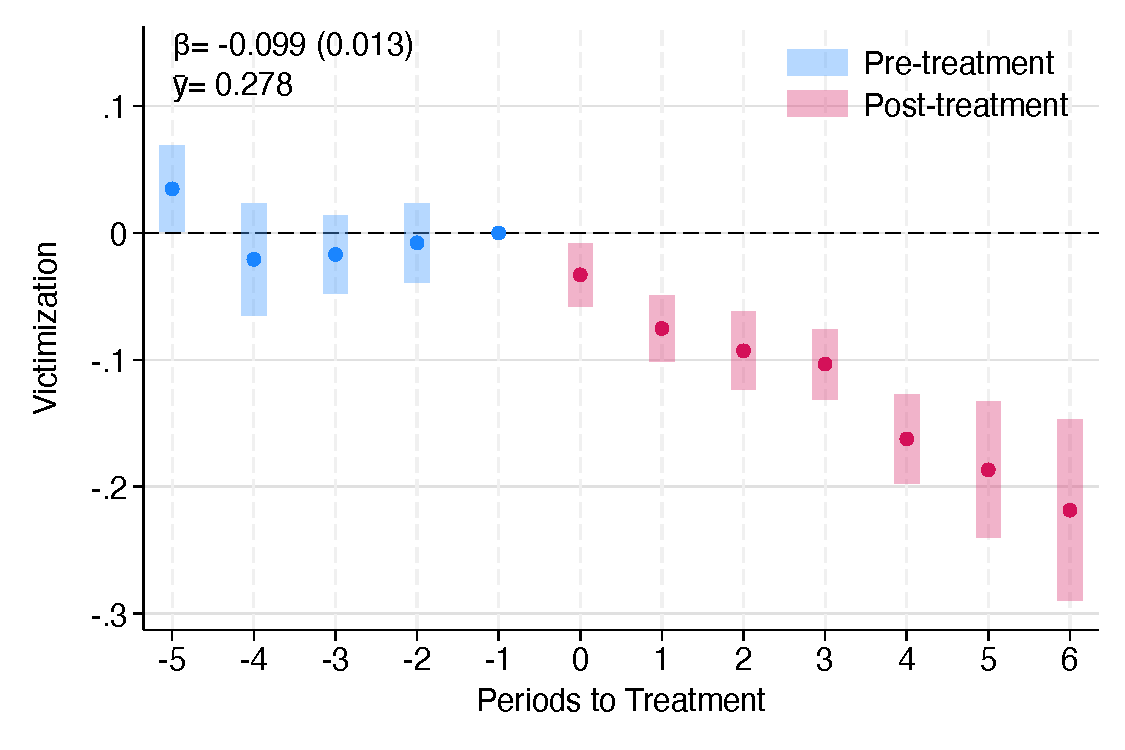
\includegraphics[width=\textwidth]{../manuscript/Graphs/results_victimization.pdf}
        \caption{Victimization in last 12 months}
    \end{subfigure}%
    ~
    \begin{subfigure}{0.495\textwidth}
    \centering
    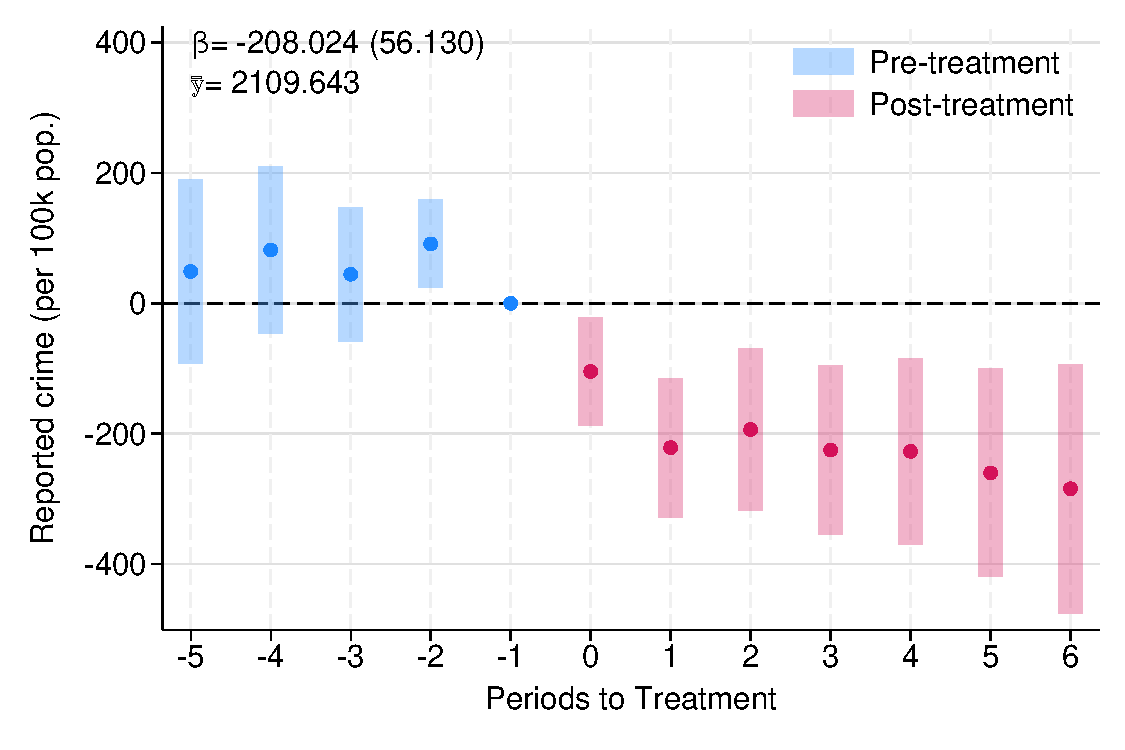
\includegraphics[width=\textwidth]{../manuscript/Graphs/totalreportedcrime_allcomunas.pdf}
        \caption{Reported crime per 100k inhabitants}
    \end{subfigure}
        \begin{subfigure}{0.495\textwidth}
        \centering
        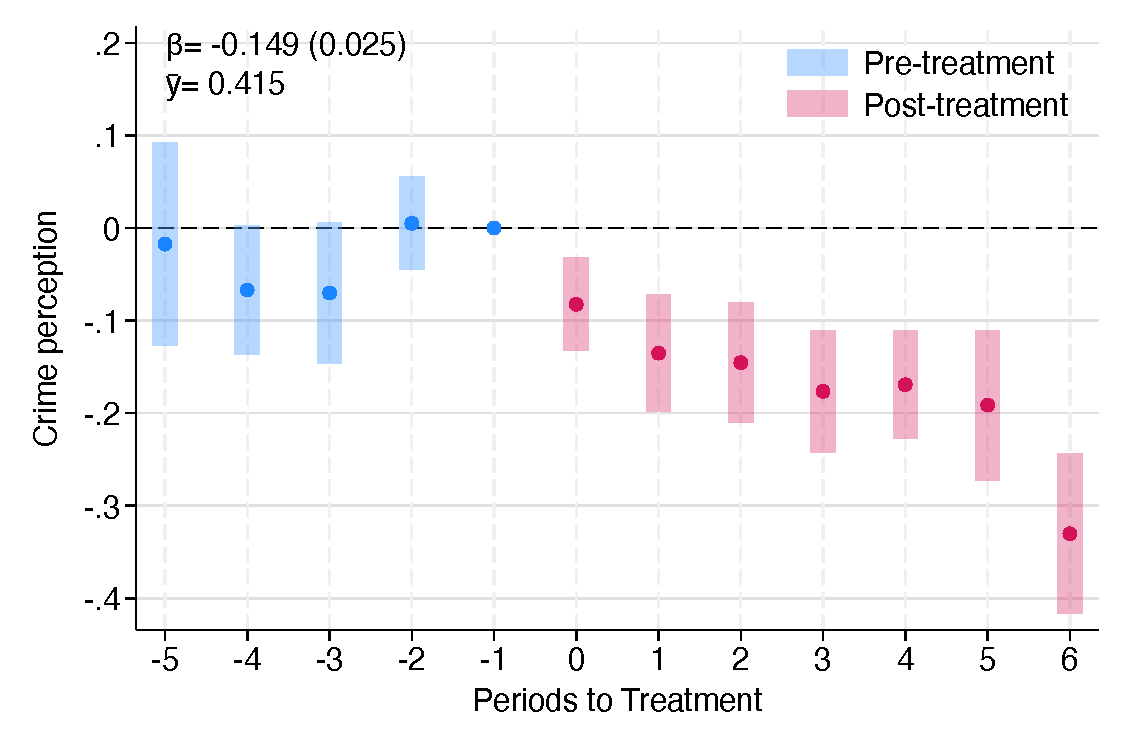
\includegraphics[width=\textwidth]{../manuscript/Graphs/results_perception.pdf}
        \caption{Households reporting an increase in crime}
    \end{subfigure}%
    ~
    \begin{subfigure}{0.495\textwidth}
    \centering
    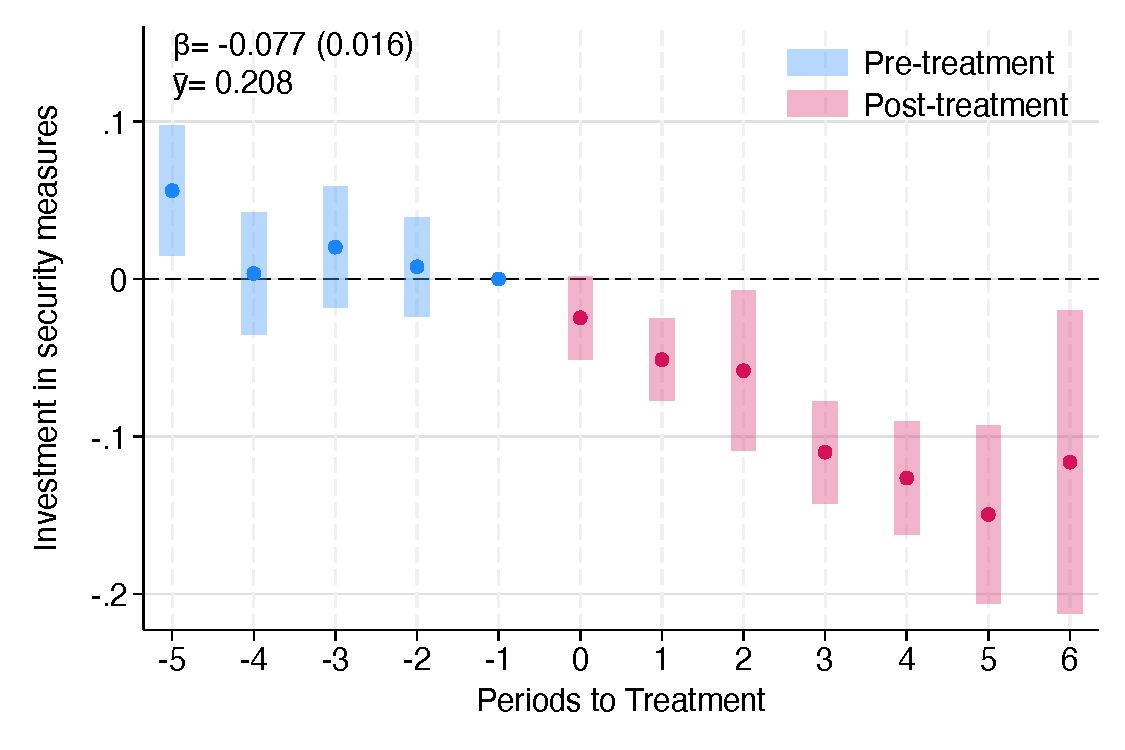
\includegraphics[width=\textwidth]{../manuscript/Graphs/results_hhprotectionmeasures.pdf}
        \caption{Households adopting security measures}
    \end{subfigure}
    \\[12pt]
    \begin{minipage}{0.99\textwidth}
    \footnotesize
    Notes: This figure shows the dynamic effects of the \emph{Plan Cuadrante} on different measures of police effectiveness. The estimation is conducted using the procedure developed in \citet{Callaway} for difference-in-differences with staggered treatment adoption. The dots in the figure represent the estimated coefficients and the bars behind them 95\% confidence intervals. Standard errors are clustered at the municipality level using the wild bootstrapping procedure. The pooled effect and the mean outcome before the introduction of the treatment is also presented in each panel. Panel (a) reports the effect of \emph{Plan Cuadrante} on the probability of household victimization in the last 12 months using the ENUSC survey. Panel (b) reports the effect on the number of crimes reported to the police in the municipality per 100,000 inhabitants using administrative data. Panel (c) reports the effect on the probability of perceiving an increase in crime using the ENUSC survey. Panel (d) reports the effect on the probability of adopting security measures in the last twelve months using the ENUSC survey. Panel (a) includes 93,041 observations; panel (b), 4,231; panel (c), 89,578; and panel (d), 93,041 observations.
    \end{minipage}
\end{figure}
}

\clearpage

{\renewcommand{\thetable}{B.3}
\begin{table}[h!]\centering
\caption{Effects of \emph{Plan Cuadrante} Controlling for Police Resources}
\label{tab:results_controlbyresources}
\resizebox{\textwidth}{!}{
\begin{threeparttable}
\begin{tabular}{l ccccc}
\toprule
 & (1) & (2) & (3) & (4) & (5) \\
\midrule
\multicolumn{6}{l}{\textit{Panel A. Victimization}} \\[0.2em]
ATT &       -0.099*** &       -0.077*** &       -0.086** &       -0.094*** &       -0.087* \\
  & (0.013) & (0.013) & (0.043) & (0.028) & (0.053) \\
N &    93,041 &    53,973 &    53,553 &    72,017 &    53,553 \\[0.4em]
\multicolumn{6}{l}{\textit{Panel B. Crime perception}} \\[0.2em]
ATT &       -0.149*** &       -0.140*** &       -0.112** &       -0.082** &       -0.111 \\
  & (0.025) & (0.032) & (0.057) & (0.033) & (0.106) \\
N &    89,578 &    52,160 &    51,746 &    69,434 &    51,746 \\[0.4em]
\multicolumn{6}{l}{\textit{Panel C. Investment in security measures}} \\[0.2em]
ATT &       -0.077*** &       -0.066*** &       -0.109*** &       -0.081*** &       -0.168*** \\
  & (0.016) & (0.019) & (0.041) & (0.019) & (0.064) \\
N &    93,041 &    53,973 &    53,553 &    72,017 &    53,553 \\[0.4em]
\multicolumn{6}{l}{\textit{Panel D. Reported crime (per 100k pop.)}} \\[0.2em]
ATT &     -208.024*** &     -190.446*** &       29.230 &     -261.439 &     -245.555 \\
  & (56.130) & (67.908) & (147.261) & (170.954) & (165.221) \\
N &     4,231 &     1,918 &     1,911 &     2,248 &     1,911 \\[0.4em]
\midrule
Sample                   & Full & Resource yrs & Resource yrs & Resource yrs & Resource yrs \\
Police officers (per 100k pop.) &      &            & \checkmark &            & \checkmark \\
Patrol vehicles (per 100k pop.) &      &            &            & \checkmark & \checkmark \\
\bottomrule
\end{tabular}
\begin{tablenotes}[flushleft]
\item \footnotesize{Note: ATT estimates of the effect of \emph{Plan Cuadrante} on each outcome. Column (1) is the baseline (full estimation sample, no controls) and reproduces the headline estimate of the corresponding estimator. Column (2) restricts the estimation to 2006--2012, the window over which police resources are observed, without including any control variable. Columns (3)--(5) add time-varying controls for police resources per 100{,}000 inhabitants: officers only; patrol vehicles only; and officers and patrol vehicles jointly (entered as separate regressors). Columns (3) and (5) cover 2006--2012, the years for which the number of officers is observed; column (4) also includes 2005, the first year for which patrol vehicles are observed. Patrol vehicles are measured, per 100{,}000 inhabitants, as all patrol automobiles (radiopatrulla, auto patrullero, auto policial, automovil, station wagon, jeep and camioneta) plus motorcycles. Standard errors in parentheses; row N reports the estimation-sample size. Estimation follows \citet{Callaway}; standard errors clustered at the municipality level using wild bootstrapping procedures. $^{*}p<0.1$, $^{**}p<0.05$, $^{***}p<0.01$.}
\end{tablenotes}
\end{threeparttable}}
\end{table}
}

\clearpage

{\renewcommand{\thefigure}{B.3}
\begin{figure}[h!]
    \centering
    \caption{Effects of \emph{Plan Cuadrante} by Resource Increase: Trust, Complaints, and Arrests}
    \label{fig:heterogeneity_appendix}
    \begin{subfigure}[t]{0.48\textwidth}
        \centering
        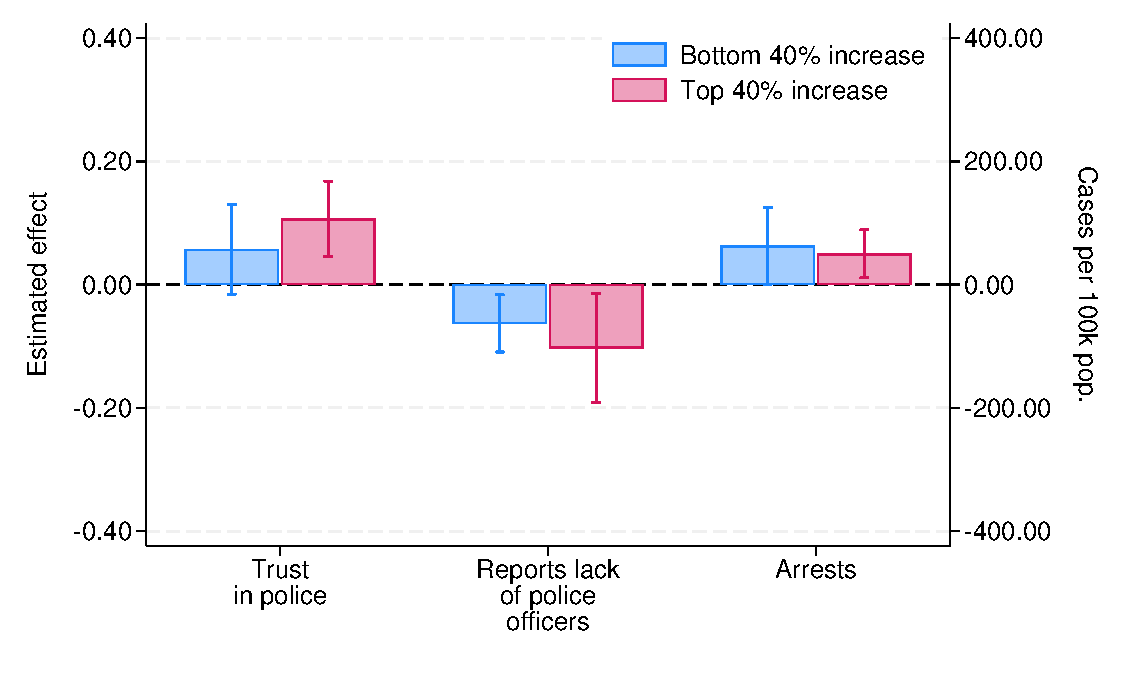
\includegraphics[width=\linewidth]{../manuscript/Graphs/heterogeneity_off_appendix.pdf}
        \caption{By the intensity of $\Delta$ in police officers}
    \end{subfigure}\hfill
    \begin{subfigure}[t]{0.48\textwidth}
        \centering
        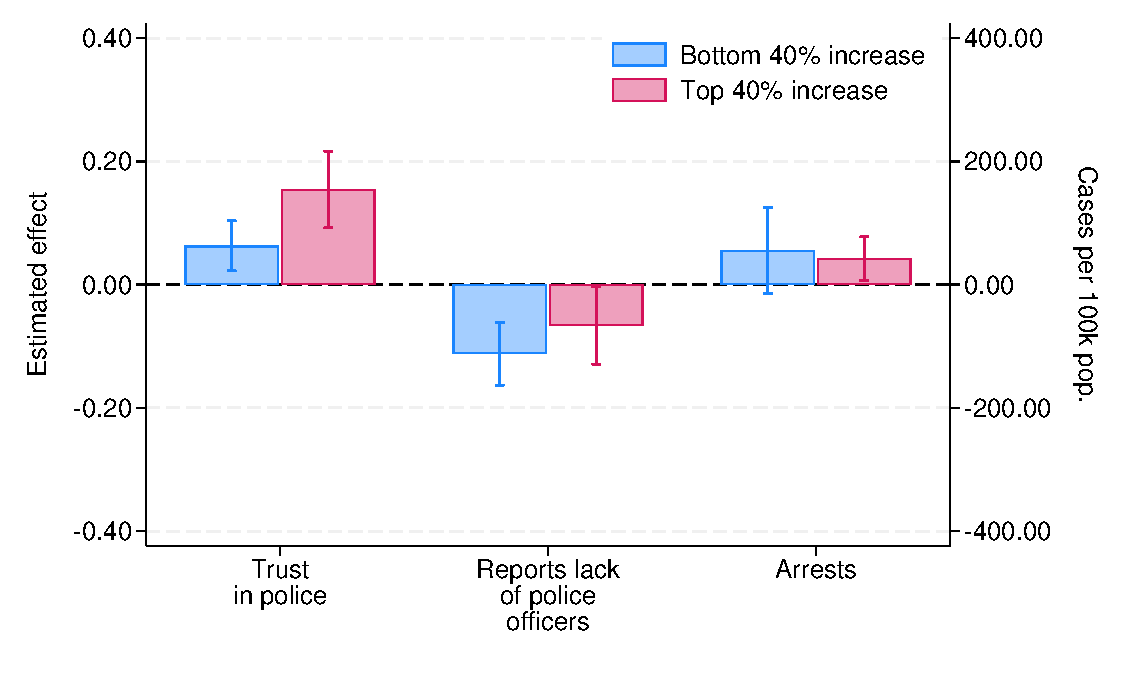
\includegraphics[width=\linewidth]{../manuscript/Graphs/heterogeneity_pv_appendix.pdf}
        \caption{By the intensity of $\Delta$ in patrol vehicles}
    \end{subfigure}
    \\[8pt]
    \begin{minipage}{0.99\textwidth}
    \footnotesize Notes: This figure complements Figure \ref{fig:figure_resources} by reporting, for the three outcomes not shown there, the effect of \emph{Plan Cuadrante} estimated separately for municipalities in the bottom 40\% (blue) and top 40\% (red) of the resource-increase distribution. Panel (a) splits municipalities by the increase in police officers and panel (b) by the increase in patrol vehicles. In each panel, arrests (administrative data, in cases per 100,000 inhabitants) are read on the right axis; the other two outcomes, from the ENUSC survey (trust in the police, and reports about the lack of police officers), are read on the left axis. Effects are estimated using the difference-in-differences estimator for staggered treatment adoption developed in \citet{Callaway}; bars are point estimates and whiskers 95\% confidence intervals, with standard errors clustered at the municipality level using the wild bootstrapping procedure.
    \end{minipage}
\end{figure}
}

\clearpage

{\renewcommand{\thefigure}{B.4}
\begin{figure}[h!]
    \centering
    \caption{Effects of \textit{Seguridad Ciudadana} on Crime Outcomes and Security Perceptions}
    \label{fig:figureA5}
    
    % Primera fila: panel (a) y (b)
    \begin{subfigure}{0.495\textwidth}
        \centering
        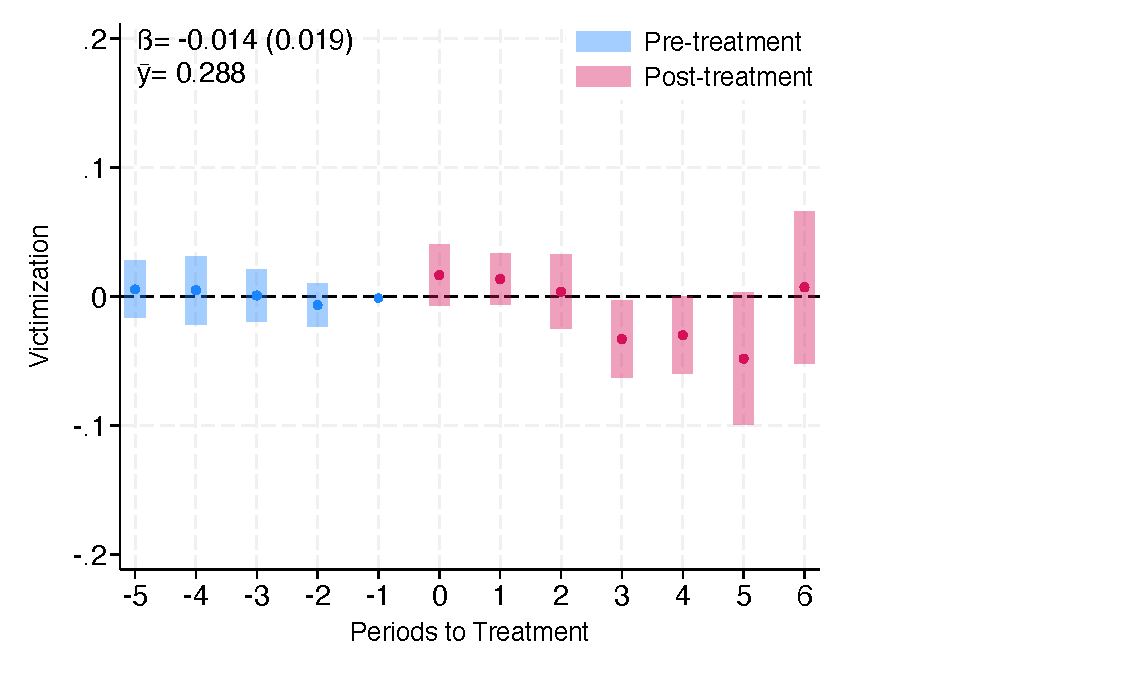
\includegraphics[width=\textwidth]{../manuscript/Graphs/results_victimization_SC.pdf}
        \caption{Victimization in last 12 months}
    \end{subfigure}%
    \hfill
    \begin{subfigure}{0.495\textwidth}
        \centering
        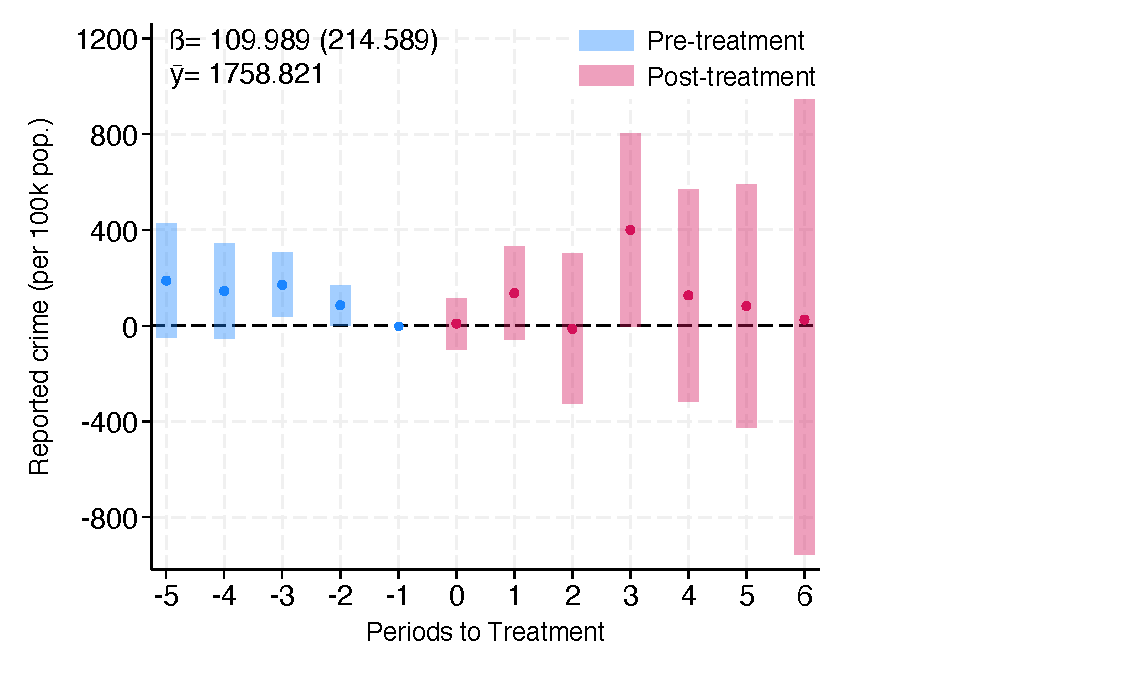
\includegraphics[width=\textwidth]{../manuscript/Graphs/totalreportedcrime_allcomunas_SC.pdf}
        \caption{Reported crime per 100k inhabitants}
    \end{subfigure}

    \vspace{12pt} % Espacio entre filas
    
    % Segunda fila: panel (c) y (d)
    \begin{subfigure}{0.495\textwidth}
        \centering
        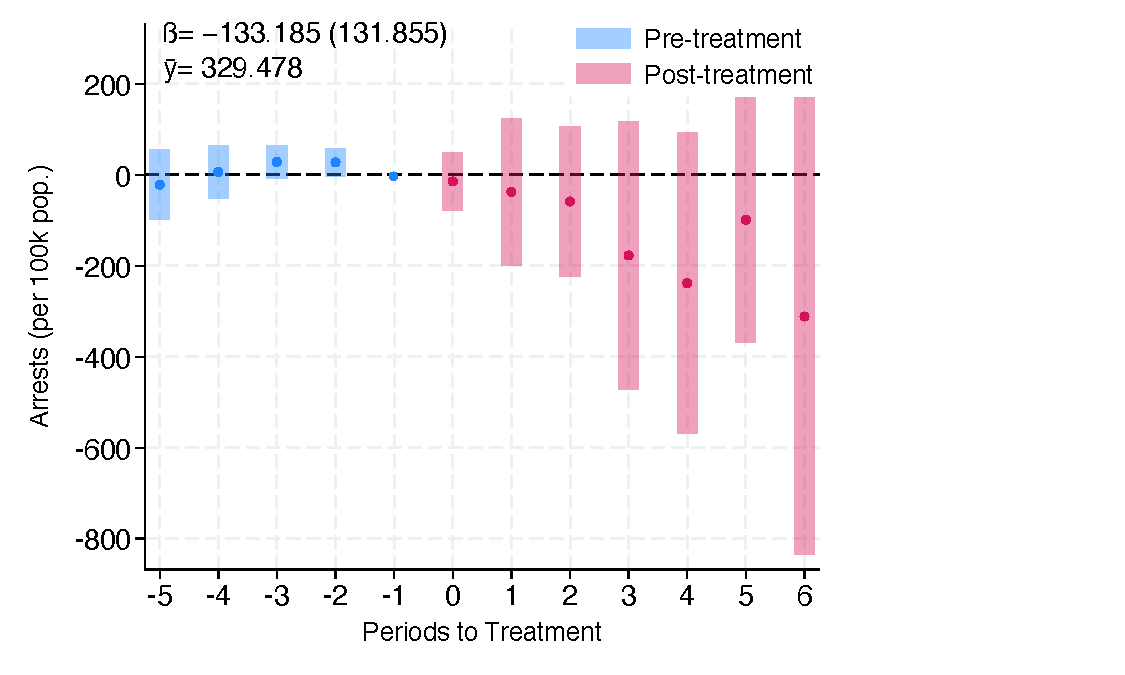
\includegraphics[width=\textwidth]{../manuscript/Graphs/totalarrestscrime_allcomunas_SC.pdf}
        \caption{Arrests per 100k inhabitants}
    \end{subfigure}%
    \hfill
    \begin{subfigure}{0.495\textwidth}
        \centering
        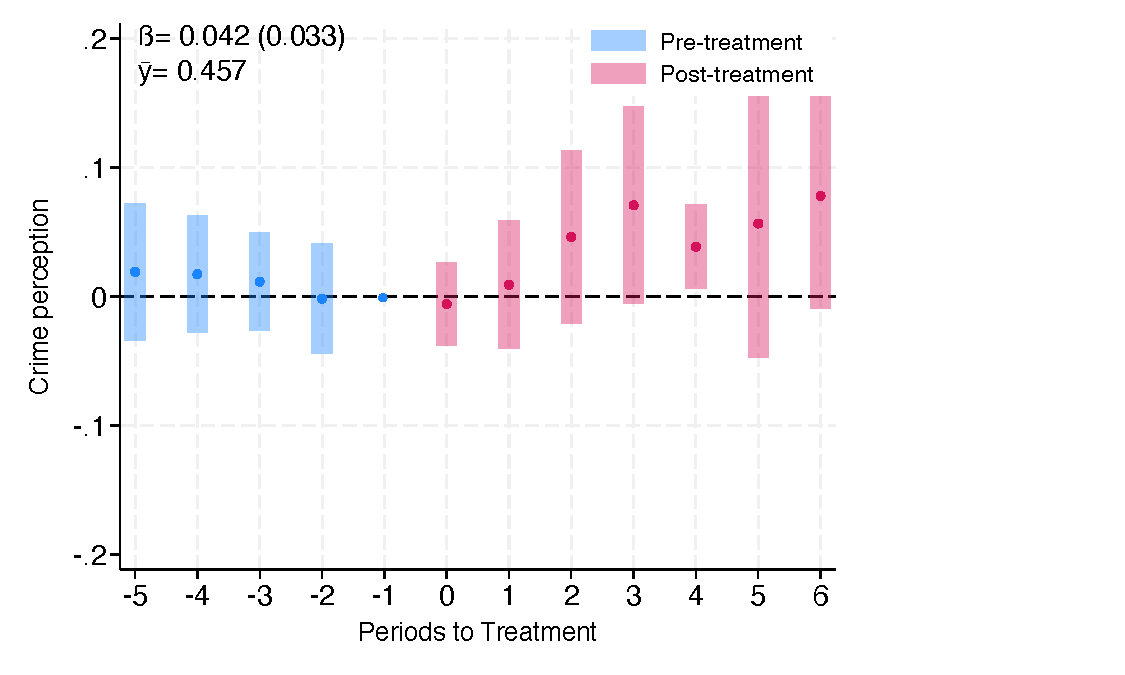
\includegraphics[width=\textwidth]{../manuscript/Graphs/results_perception_SC.pdf}
        \caption{Households reporting an \\ increase in crime}
    \end{subfigure}
    
    \vspace{12pt} % Espacio entre filas
    
    % Tercera fila: panel (e)
    \begin{subfigure}{0.495\textwidth}
        \centering
        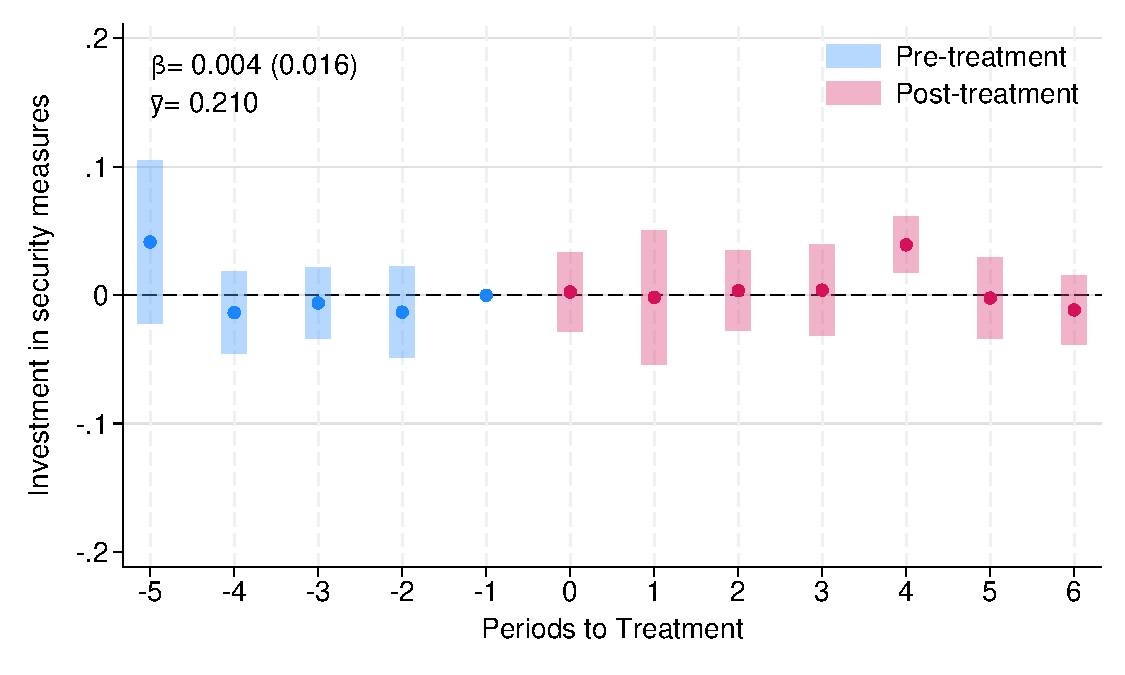
\includegraphics[width=\textwidth]{../manuscript/Graphs/results_hhprotectionmeasures_SC.pdf}
        \caption{Households adopting security measures}
    \end{subfigure}

    \vspace{12pt} % Espacio para las notas
    
    \begin{minipage}{0.99\textwidth}
        \footnotesize
        Notes: This figure shows the dynamic effects of the \textit{Seguridad Ciudadana} program on different measures of crime and security perceptions. The estimation is conducted using the procedure developed in \citet{Callaway} for difference-in-differences with staggered treatment adoption. The dots in the figure represent the estimated coefficients and the bars behind them 95\% confidence intervals. Standard errors are clustered at the municipality level using wild bootstrapping. The pooled effect and the mean outcome before the introduction of the treatment for the outcome---computed as in Figure \ref{fig:figure02}, using only the pre-treatment observations of treated units---is also presented in each panel. Panel (a) reports the effect of \textit{Seguridad Ciudadana} on the probability of household victimization in the last 12 months using the ENUSC survey. Panel (b) reports the effect on the number of crimes reported to the police in the municipality per 100,000 inhabitants using administrative data. Panel (c) reports the effect on the number of arrests in the municipality per 100,000 inhabitants using administrative data. Panel (d) reports the effect on the probability of perceiving an increase in crime using the ENUSC survey. Panel (e) reports the effect on the probability of adopting security measures in the last twelve months using the ENUSC survey. Panel (a) includes 210,102 observations; panel (b), 2,234; panel (c), 1,908; panel (d), 203,078; and panel (e), 74,316 observations.
    \end{minipage}
\end{figure}
}

\clearpage

{\renewcommand{\thefigure}{B.5}
\begin{figure}[h!]
    \centering
    \caption{Association between Police Resources and Police Effectiveness (No \emph{Plan Cuadrante} Variation)}
    \label{fig:figureA7B}
    \begin{subfigure}[t]{0.48\textwidth}
        \centering
        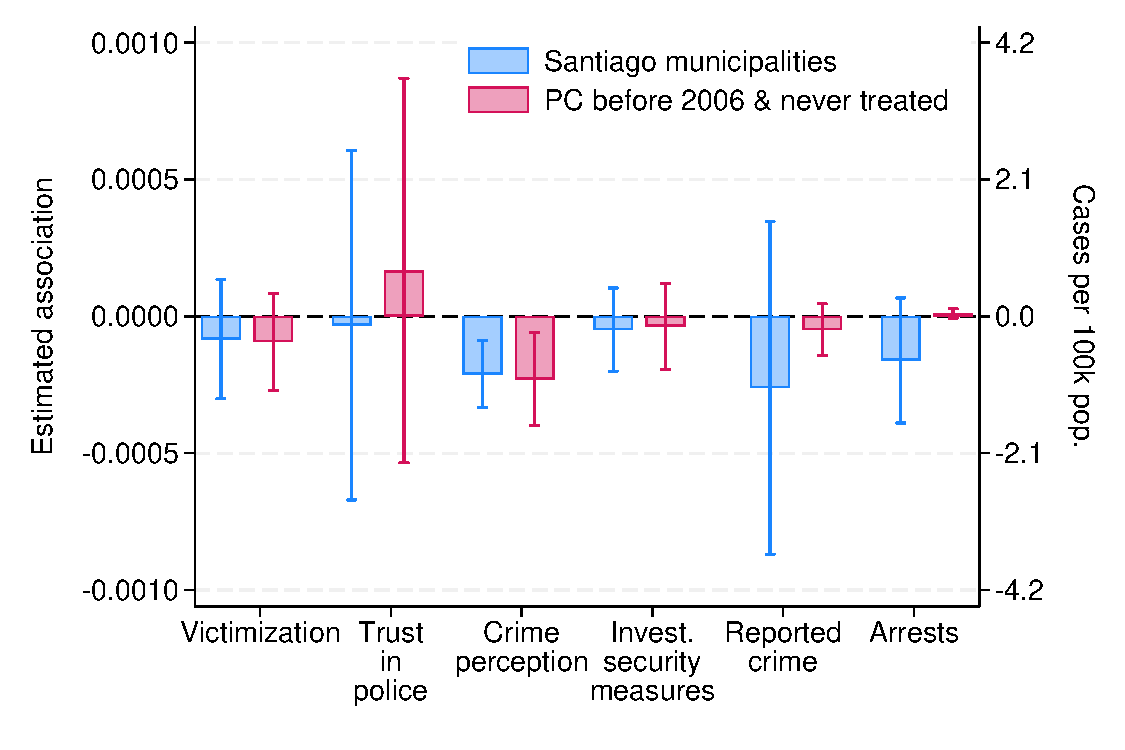
\includegraphics[width=\linewidth]{../manuscript/Graphs/results_corr_novariation_off.pdf}
        \caption{Association with police officers}
    \end{subfigure}\hfill
    \begin{subfigure}[t]{0.48\textwidth}
        \centering
        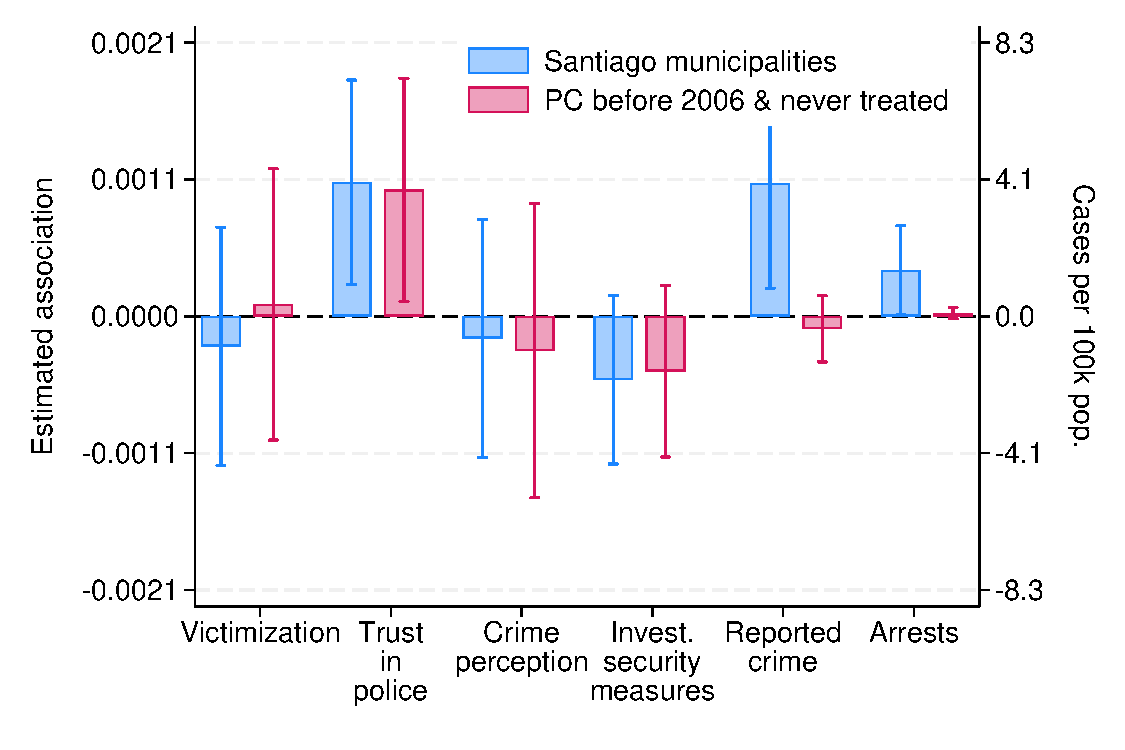
\includegraphics[width=\linewidth]{../manuscript/Graphs/results_corr_novariation_veh.pdf}
        \caption{Association with patrol vehicles}
    \end{subfigure}
    \\[10pt]
    \begin{minipage}{0.99\textwidth}
    \footnotesize Notes: The figure shows the estimated within-municipality association between police resources (per 100,000 inhabitants) and the main outcomes, in municipalities where \emph{Plan Cuadrante} does not vary over the sample period. Estimates come from OLS regressions of each outcome on the resource measure with municipality and year fixed effects; standard errors are clustered at the municipality level. Blue bars use the 41 metropolitan municipalities of Santiago, all of which adopted \emph{Plan Cuadrante} in 2000; red bars use the broader set of municipalities that adopted \emph{Plan Cuadrante} before 2006 together with the never-treated municipalities surveyed in ENUSC (2006--2012). Reported crime and arrests (administrative data, in cases per 100,000 inhabitants) are read on the right axis; all other outcomes, from the ENUSC survey (victimization, trust in the police, crime perception, and investment in security measures), are read on the left axis. Panel (a) reports associations with the number of police officers; panel (b) with the number of patrol vehicles. Bars are point estimates with 95\% confidence intervals.
    \end{minipage}
\end{figure}
}

\clearpage

{\renewcommand{\thetable}{B.4}
\begin{table}[H]
\centering
\caption{Predictors of the Increase in Police Resources under \emph{Plan Cuadrante}}
\label{tab:resourcecorrelates}
\begin{threeparttable}
\small
\setlength{\tabcolsep}{6pt}
\renewcommand{\arraystretch}{1.1}
\begin{tabular}{@{}l cc cc@{}}
\toprule
& \multicolumn{2}{c}{Administrative sample} & \multicolumn{2}{c}{ENUSC sample} \\
\cmidrule(lr){2-3} \cmidrule(lr){4-5}
& Police & Patrol & Police & Patrol \\
Dep.\ var: avg.\ annual increase & officers & vehicles & officers & vehicles \\
in resources (share of pre-adoption level) & (1) & (2) & (3) & (4) \\
\midrule
Reported crime (per 100k pop.) & $-0.203^{**}$ & $-0.199^{**}$ & $-0.319^{*}$ & $0.272^{*}$ \\
 & (0.099) & (0.097) & (0.182) & (0.137) \\
Arrests (per 100k pop.) & $0.099$ & $-0.041$ & $0.003$ & $0.297$ \\
 & (0.136) & (0.129) & (0.186) & (0.223) \\
Victimization &  &  & $-0.017^{*}$ & $-0.025^{*}$ \\
 &  &  & (0.010) & (0.013) \\
Crime perception &  &  & $0.005$ & $0.008$ \\
 &  &  & (0.017) & (0.014) \\
Trust in the police &  &  & $0.024$ & $0.027$ \\
 &  &  & (0.018) & (0.019) \\
Investment in security measures &  &  & $0.004$ & $-0.003$ \\
 &  &  & (0.010) & (0.009) \\
Police officers (per 100k pop.) & $-0.207$ & $0.155$ & $-0.888^{***}$ & $0.571^{***}$ \\
 & (0.155) & (0.129) & (0.154) & (0.136) \\
Patrol vehicles (per 100k pop.) & $-0.129$ & $-0.139$ & $0.537^{**}$ & $-0.507^{***}$ \\
 & (0.129) & (0.126) & (0.212) & (0.169) \\
Log population & $-0.529^{***}$ & $-0.203^{*}$ & $-0.193$ & $-0.626^{**}$ \\
 & (0.145) & (0.112) & (0.189) & (0.269) \\
Poverty rate (2004) & $0.170$ & $0.308^{**}$ & $0.027$ & $-0.017$ \\
 & (0.113) & (0.126) & (0.108) & (0.108) \\
\midrule
Observations & 65 & 65 & 8,781 & 8,781 \\
R-squared & 0.342 & 0.282 & 0.614 & 0.545 \\
\bottomrule
\end{tabular}
\begin{tablenotes}[flushleft]
\footnotesize
\item \textit{Note:} OLS regressions of the average annual increase in police officers (columns 1 and 3) and patrol vehicles (columns 2 and 4) per 100{,}000 inhabitants, from the year before adoption of \emph{Plan Cuadrante} to 2012. As in panels (a) and (b) of Figure \ref{fig:figure_resources}, the increase is expressed as a share of the resources available the year before adoption. Columns 1--2 use the administrative sample at the municipality level; columns 3--4 use ENUSC survey respondents interviewed before 2007 (survey outcomes at the respondent level, other regressors as pre-2006 municipality aggregates). All variables are standardized. Standard errors clustered by municipality in parentheses.
\item $^{*}p<0.1$; $^{**}p<0.05$; $^{***}p<0.01$.
\end{tablenotes}
\end{threeparttable}
\end{table}
}

\clearpage

{\renewcommand{\thefigure}{B.6}
\begin{figure}[H]
    \centering
    \caption{Timing of Adoption of \emph{Plan Cuadrante} and Perceived Police Performance}
    \label{fig:balance_doseresponse}
    \begin{subfigure}{0.495\textwidth}
        \centering
        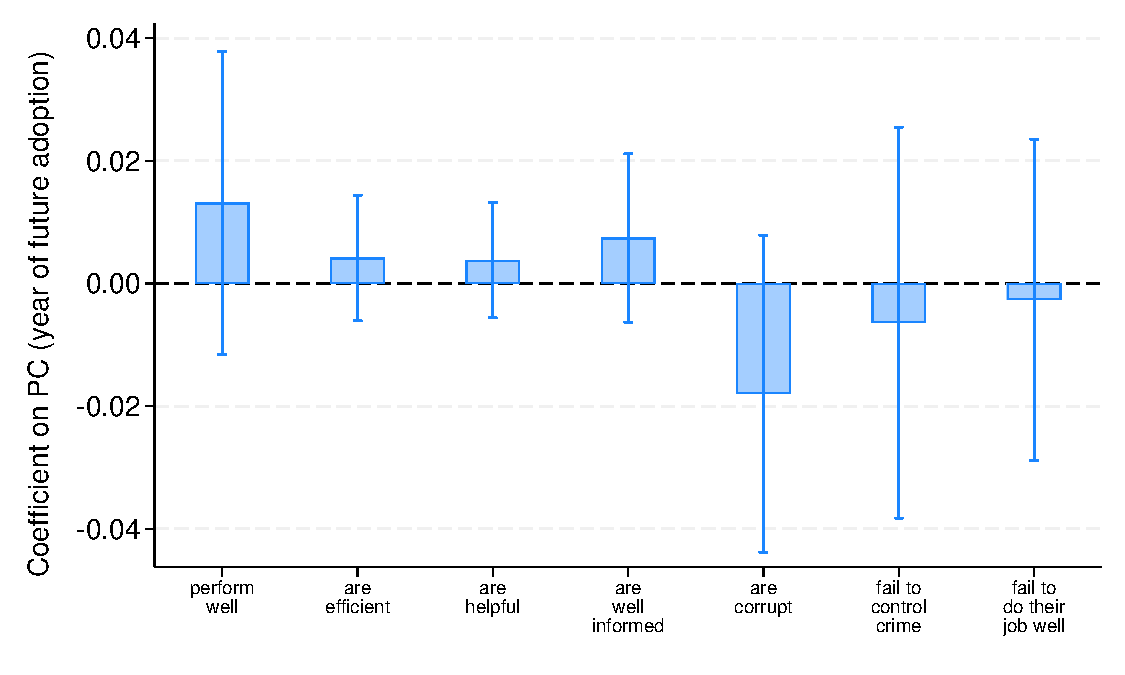
\includegraphics[width=\textwidth]{../manuscript/Graphs/balance_carabperc.pdf}
        \caption{Year of adoption and police performance before adoption}
    \end{subfigure}%
    ~
    \begin{subfigure}{0.495\textwidth}
        \centering
        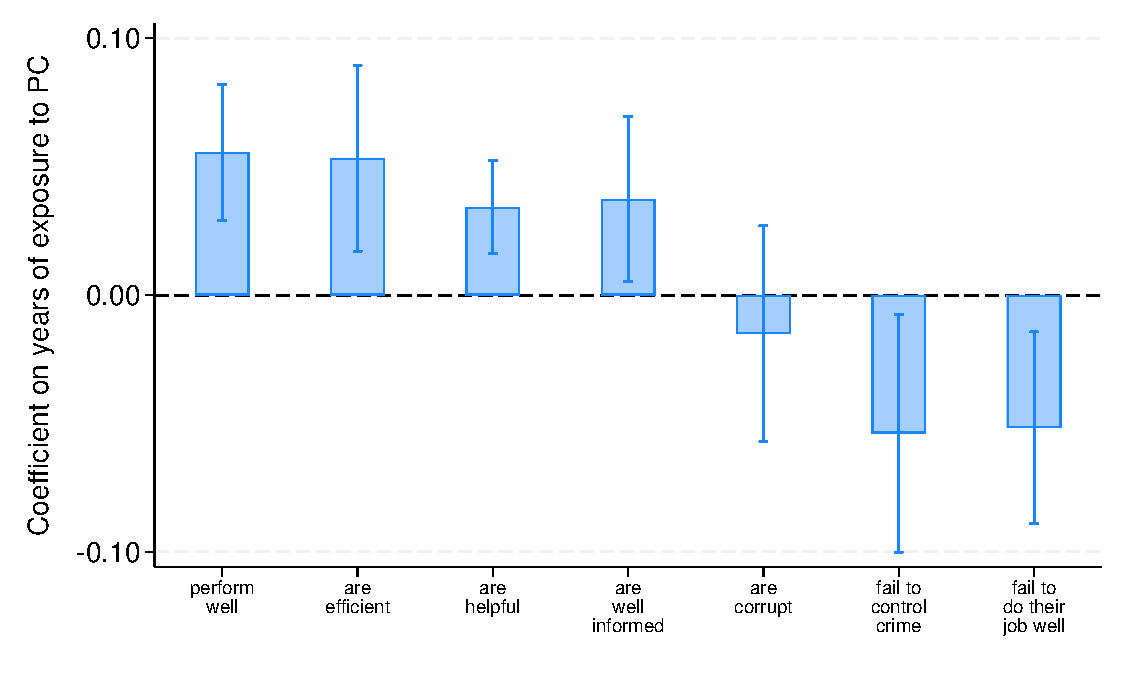
\includegraphics[width=\textwidth]{../manuscript/Graphs/doseresponse_carabperc.pdf}
        \caption{Years exposed to \emph{Plan Cuadrante} (dose response)}
    \end{subfigure}%
    \\[12pt]
    \begin{minipage}{0.99\textwidth}
    Notes: The figure considers seven measures of police performance: the share of respondents who perceive police performance as good, and who perceive the police to be efficient, helpful, well informed, corrupt, failing to control crime, and failing to do their job well. Using the sample of municipalities that adopted \emph{Plan Cuadrante} after 2005, panel (a) examines whether the future timing of adoption of \emph{Plan Cuadrante} is correlated with perceived police performance in 2005, before the introduction of the program. Panel (b) reestimates the same comparison as Figure \ref{fig:figure05}, replacing the binary adoption indicator with the municipality's number of years of exposure to \emph{Plan Cuadrante} as of 2005. In both panels, each bar plots the coefficient from a separate regression of one performance measure. The graphs display the estimated coefficients and 95\% confidence intervals.
    \end{minipage}
\end{figure}
}

\clearpage

{\renewcommand{\thefigure}{C.8}
\begin{figure}[h!]
    \centering
    \caption{Effects of \emph{Plan Cuadrante} on Reported Crime and Arrests Using the Full Set of Post-treatment and Pre-treatment Periods}
    \label{fig:admin_uncapped}
    \begin{subfigure}{0.495\textwidth}
        \centering
        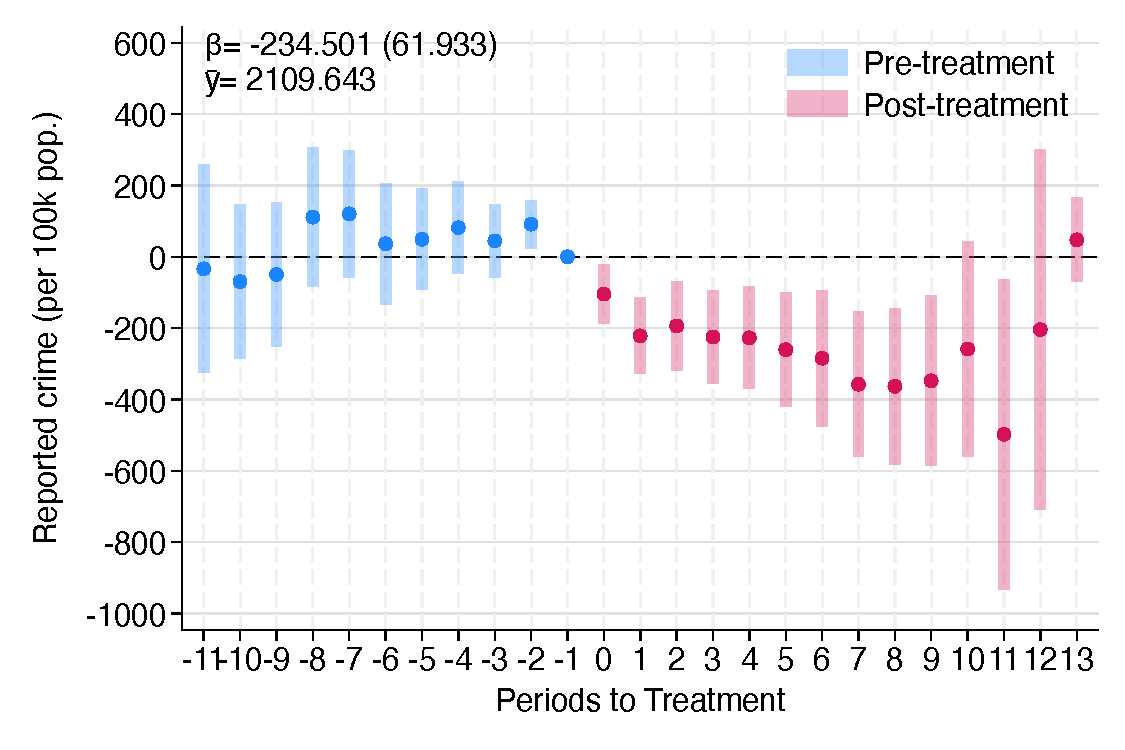
\includegraphics[width=0.98\textwidth]{../manuscript/Graphs/totalreportedcrime_allcomunas_uncapped.pdf}
        \caption{Reported crime per 100k inhabitants}
    \end{subfigure}%
    ~
    \begin{subfigure}{0.495\textwidth}
    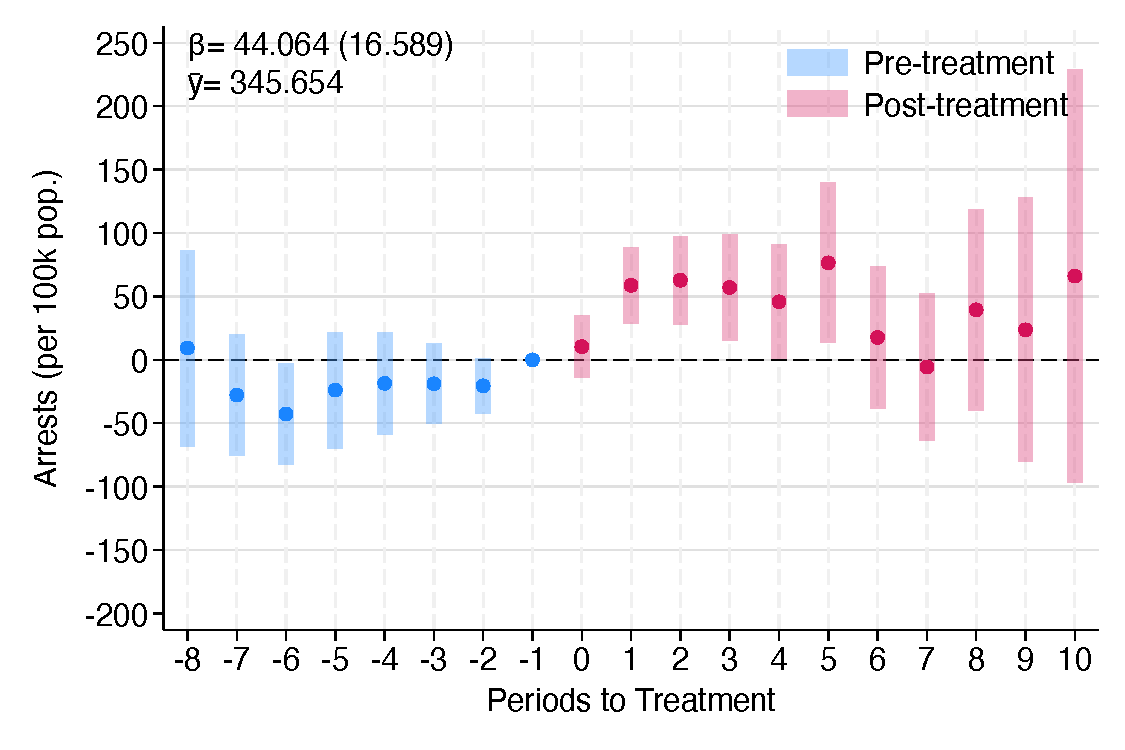
\includegraphics[width=0.98\textwidth]{../manuscript/Graphs/totalarrestscrime_allcomunas_uncapped.pdf}
        \caption{Arrests per 100k inhabitants}
    \end{subfigure}
    \begin{minipage}{\textwidth}
    \footnotesize
   Notes: This figure shows the dynamic effects of \emph{Plan Cuadrante} on the number of crimes reported to the police in the municipality per 100,000 inhabitants (panel a) and on the number of arrests in the municipality per 100,000 inhabitants (panel b), using administrative data. The estimation is conducted using the procedure developed in \citet{Callaway} for difference-in-differences with staggered treatment adoption. The dots in the figure represent the estimated coefficients and the bars behind them 95\% confidence intervals. Standard errors are clustered at the municipality level using the wild bootstrapping procedure. The pooled effect and the mean outcome before the introduction of the treatment are also presented in each panel. Unlike Figure \ref{fig:figure02} in the main text, we do not cap the event study to the same 5 pre-treatment and 6 post-treatment periods used for symmetry with the ENUSC-based analysis. Instead, we exploit the full set of post-treatment and pre-treatment periods. Panel (a) includes 4,371 observations and panel (b) 3,372 observations.
    \end{minipage}
\end{figure}
}

\clearpage

